\title{PCB Analysis}

\date{\today}

\documentclass[12pt]{article}

\usepackage{graphicx}

\begin{document}
\maketitle

\section{Computational Hardware}
\includegraphics[scale=0.1,angle=270]{images/Computation_Resources/IMG_0619.JPG}
\includegraphics[scale=0.1]{images/Computation_Resources/IMG_0620.JPG}
\includegraphics[scale=0.1]{images/Computation_Resources/IMG_0621.JPG}
\includegraphics[scale=0.1]{images/Computation_Resources/IMG_0622.JPG}
\section{Printer Path}
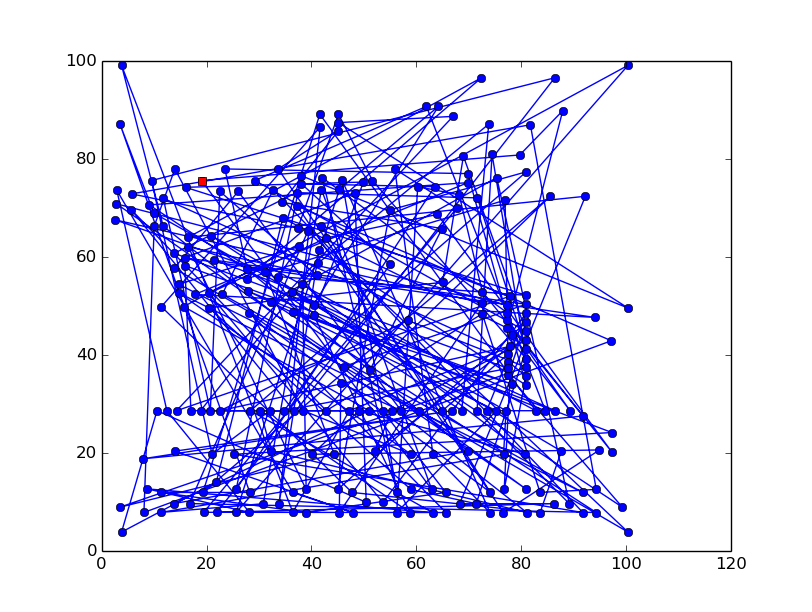
\includegraphics{images/Path/original_path.png}
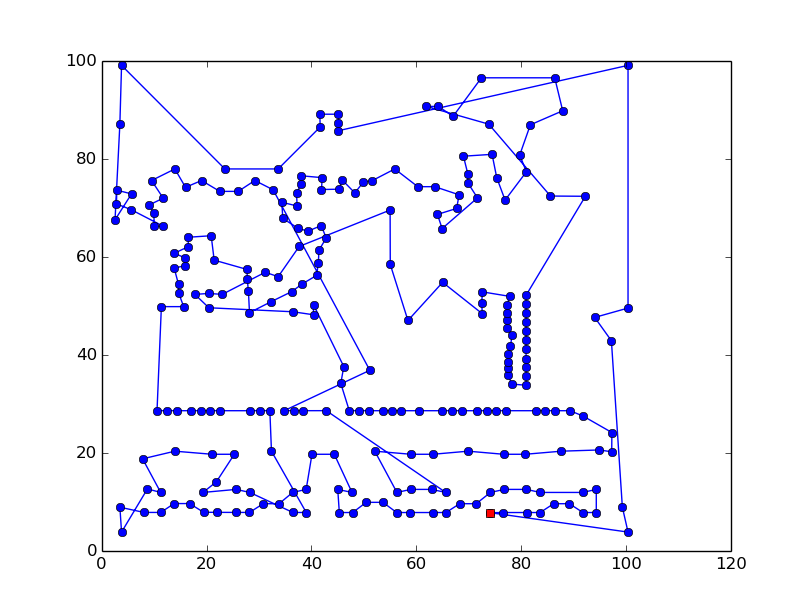
\includegraphics{images/Path/best_found_path.png}


\section{Chip Analysis Setup}
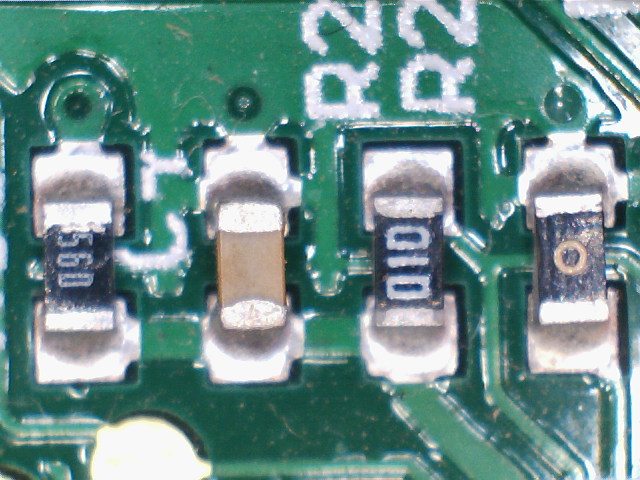
\includegraphics{images/Segmentation/raw_image.png}
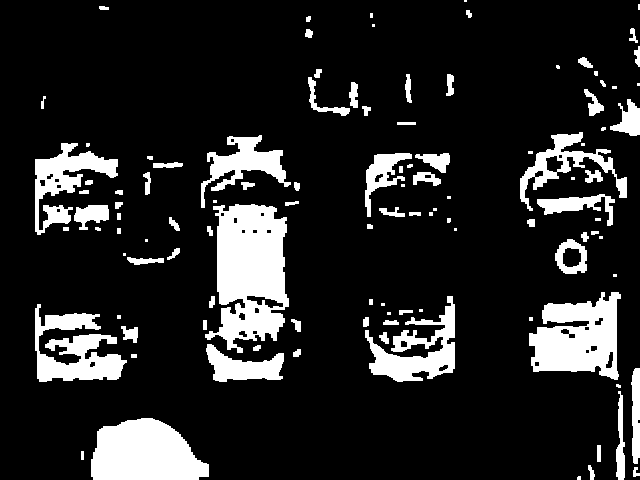
\includegraphics{images/Segmentation/binary.png}
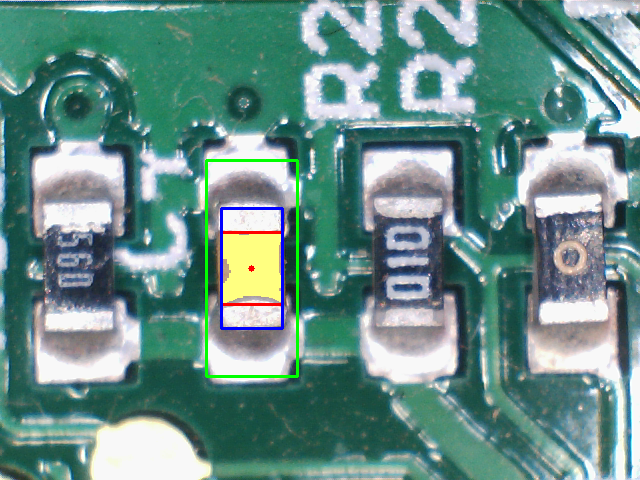
\includegraphics{images/Segmentation/part_analysis.png}


\section{Volume Analysis Setup}
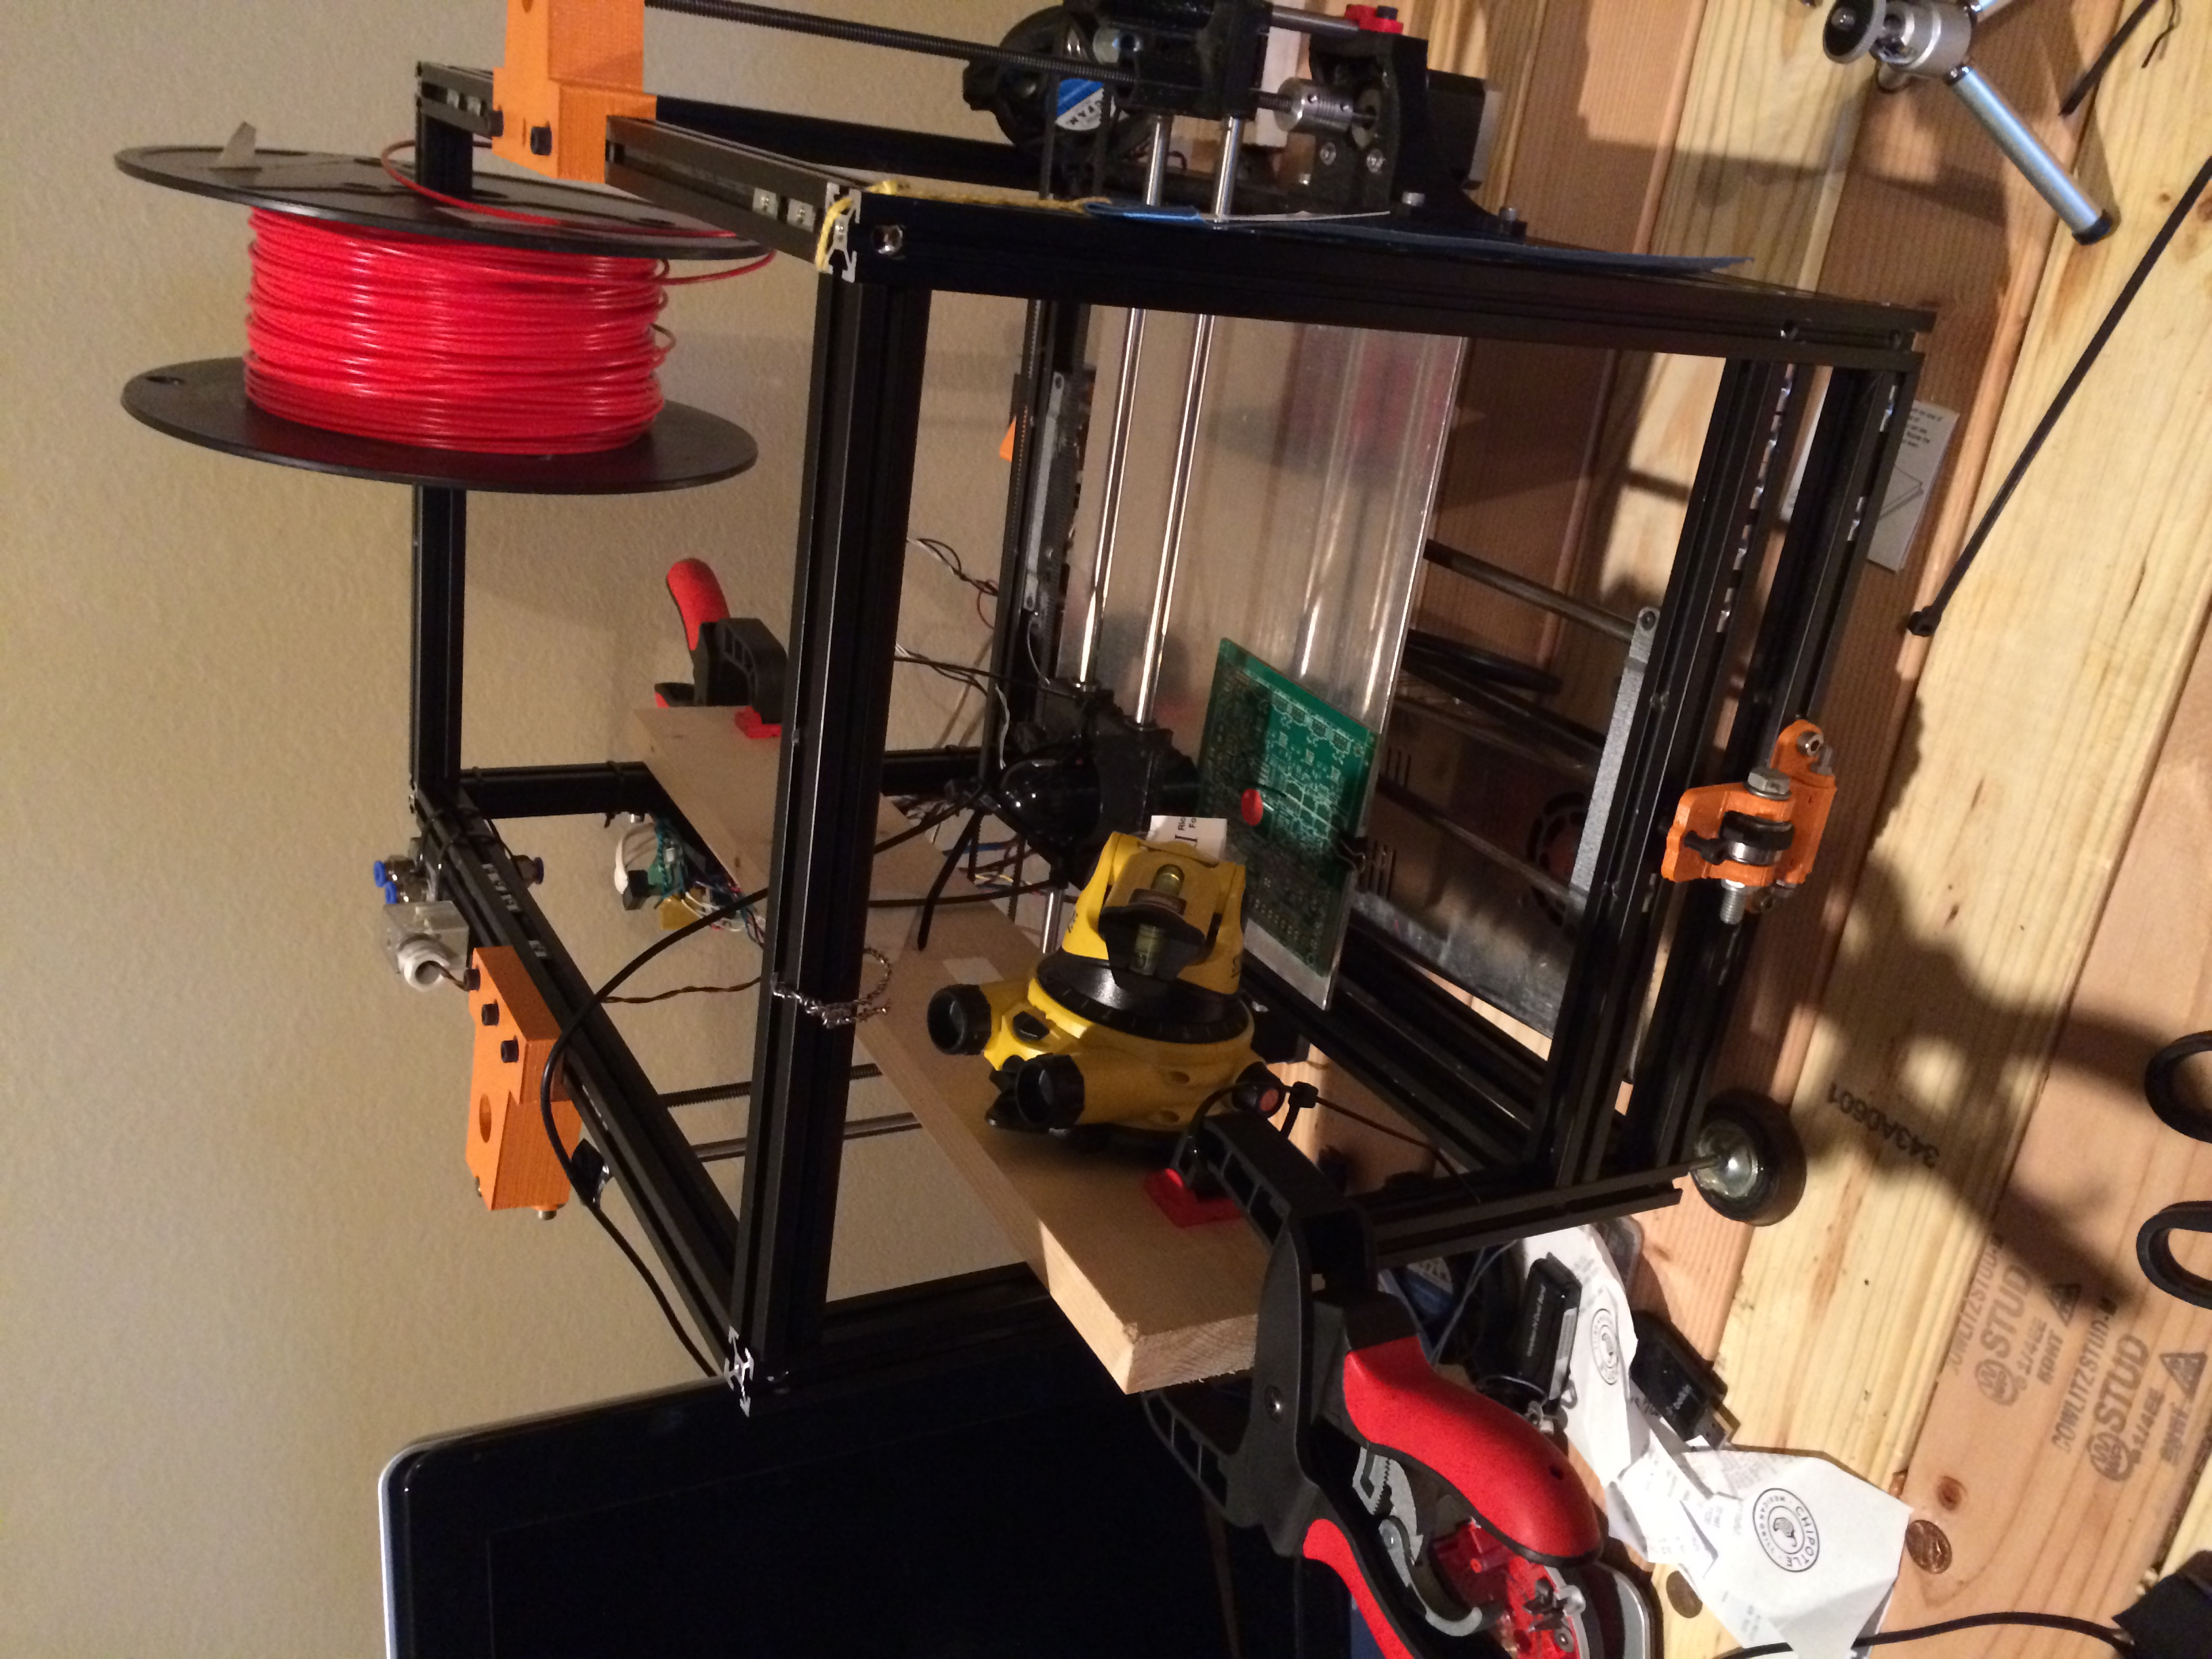
\includegraphics[scale=0.1,angle=270]{images/volume_analysis_setup/IMG_0604.JPG}
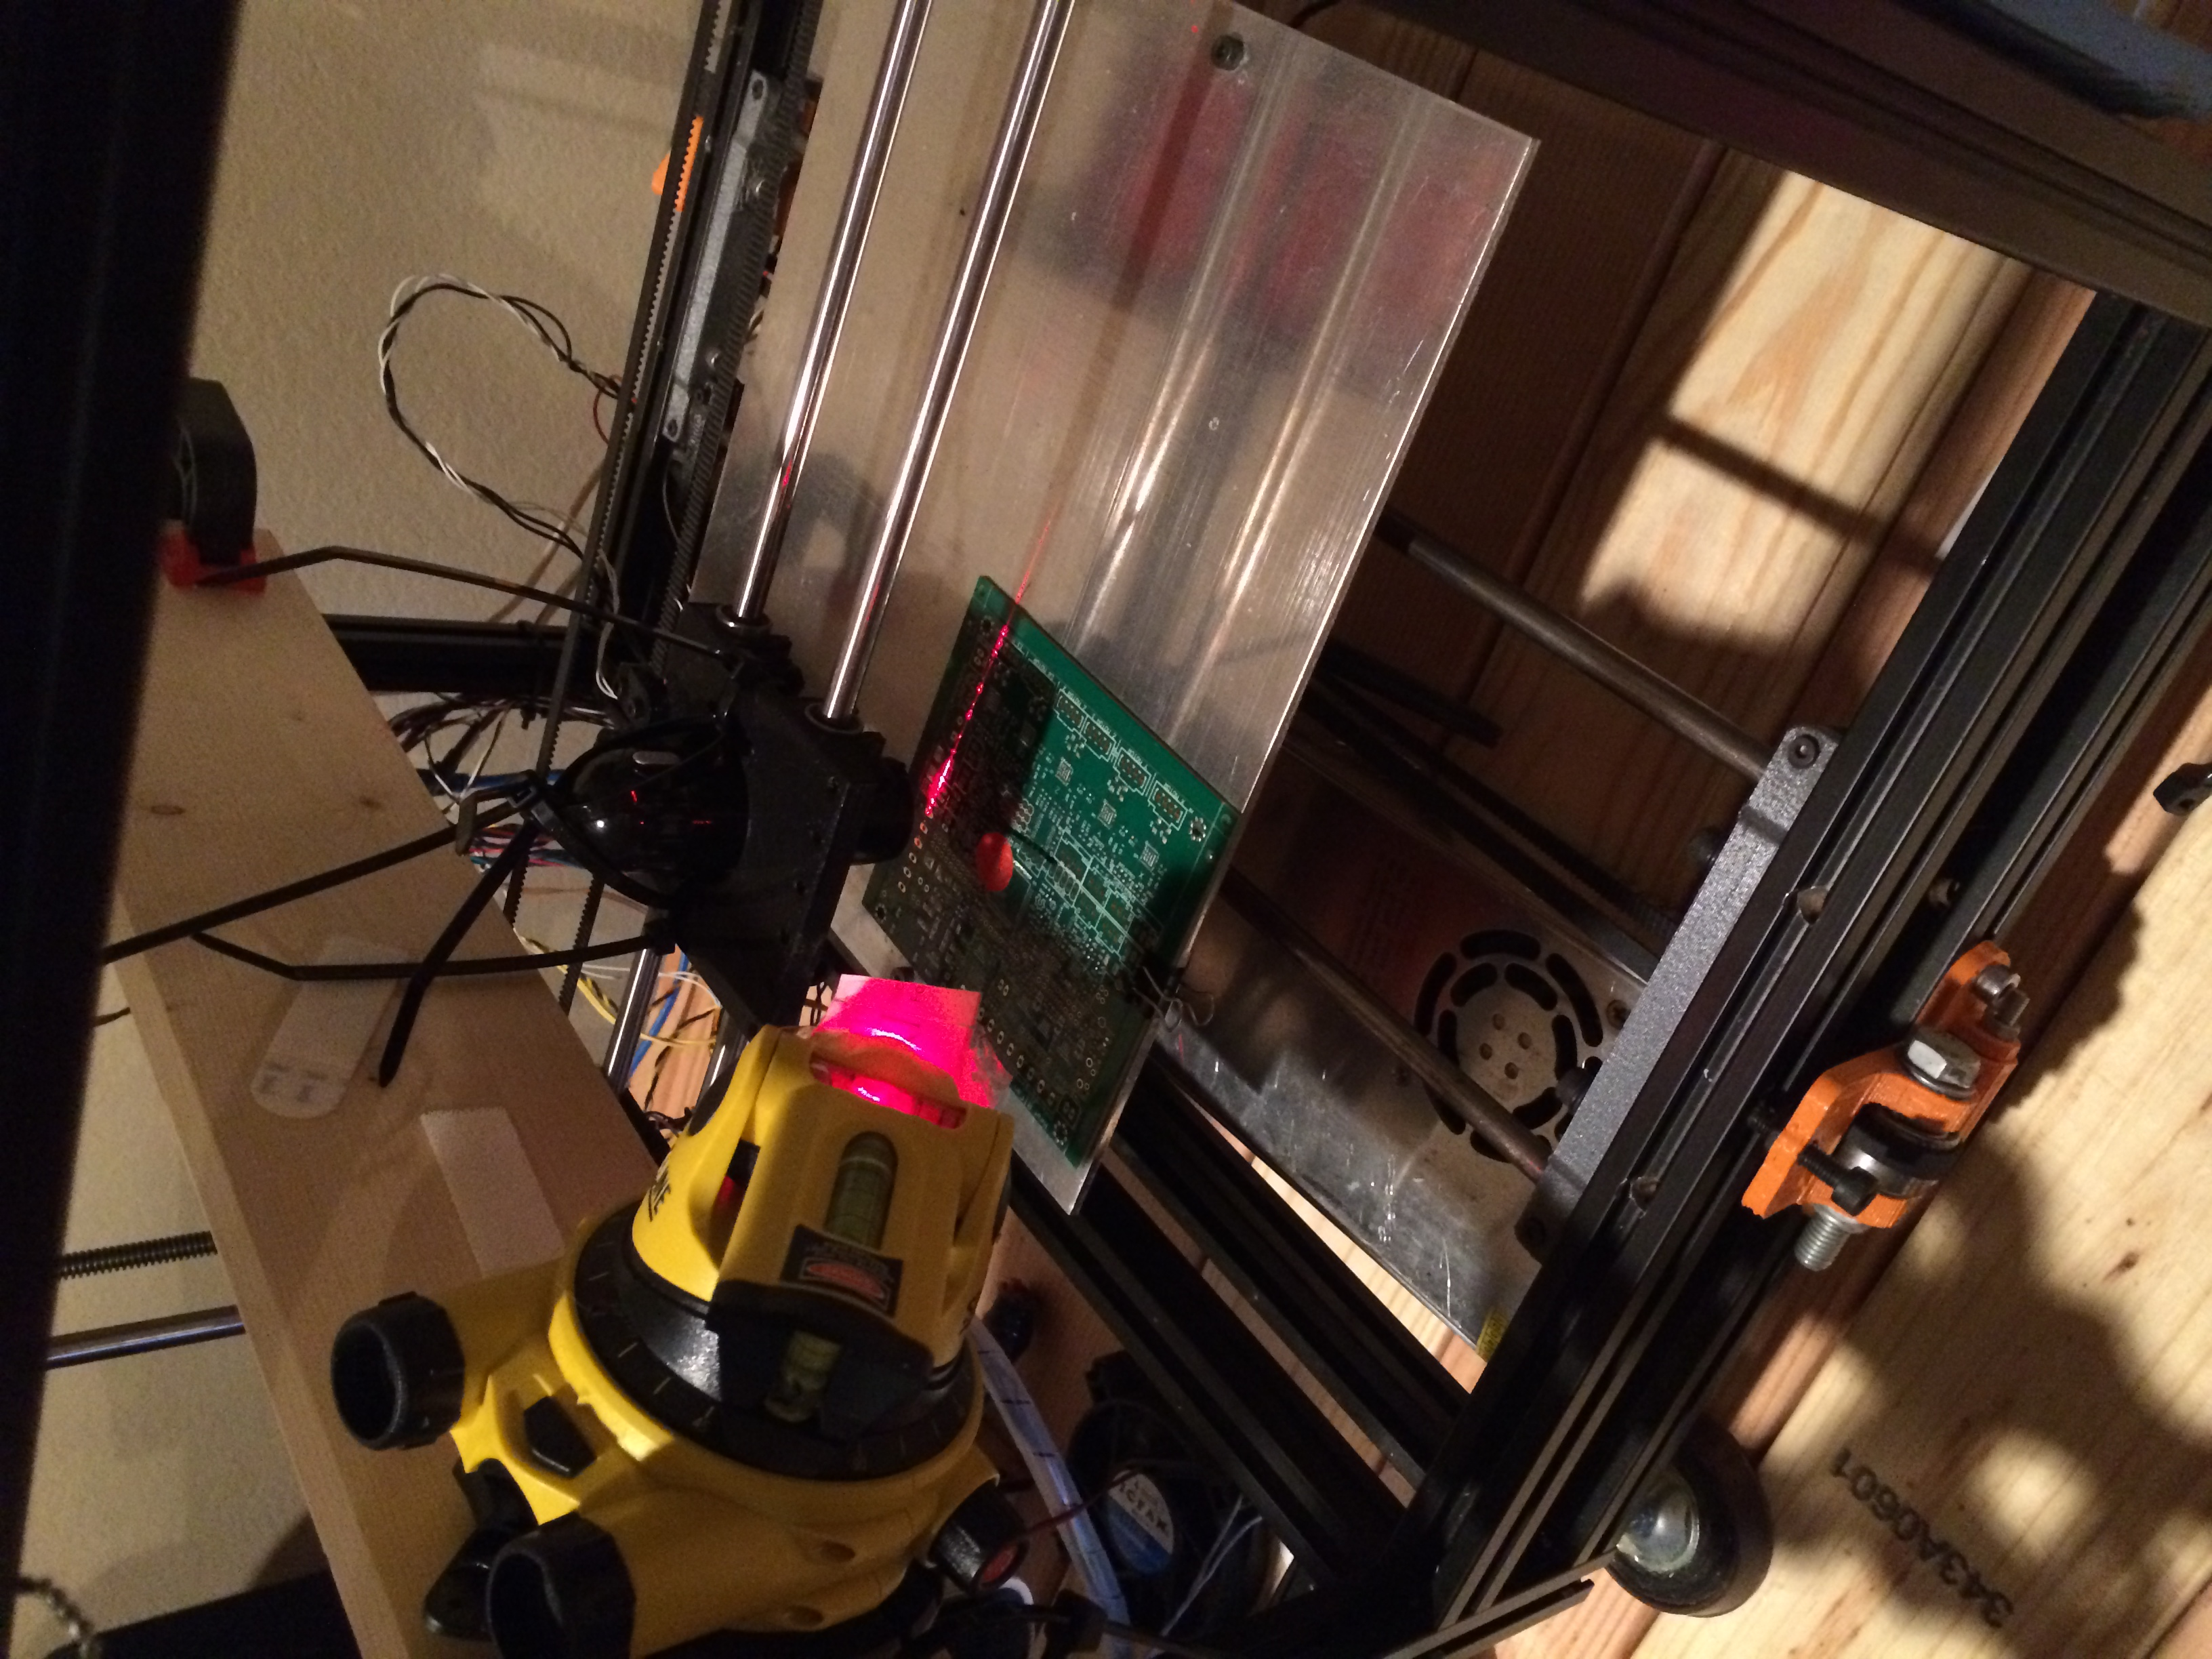
\includegraphics[scale=0.1,angle=270]{images/volume_analysis_setup/IMG_0605.JPG}
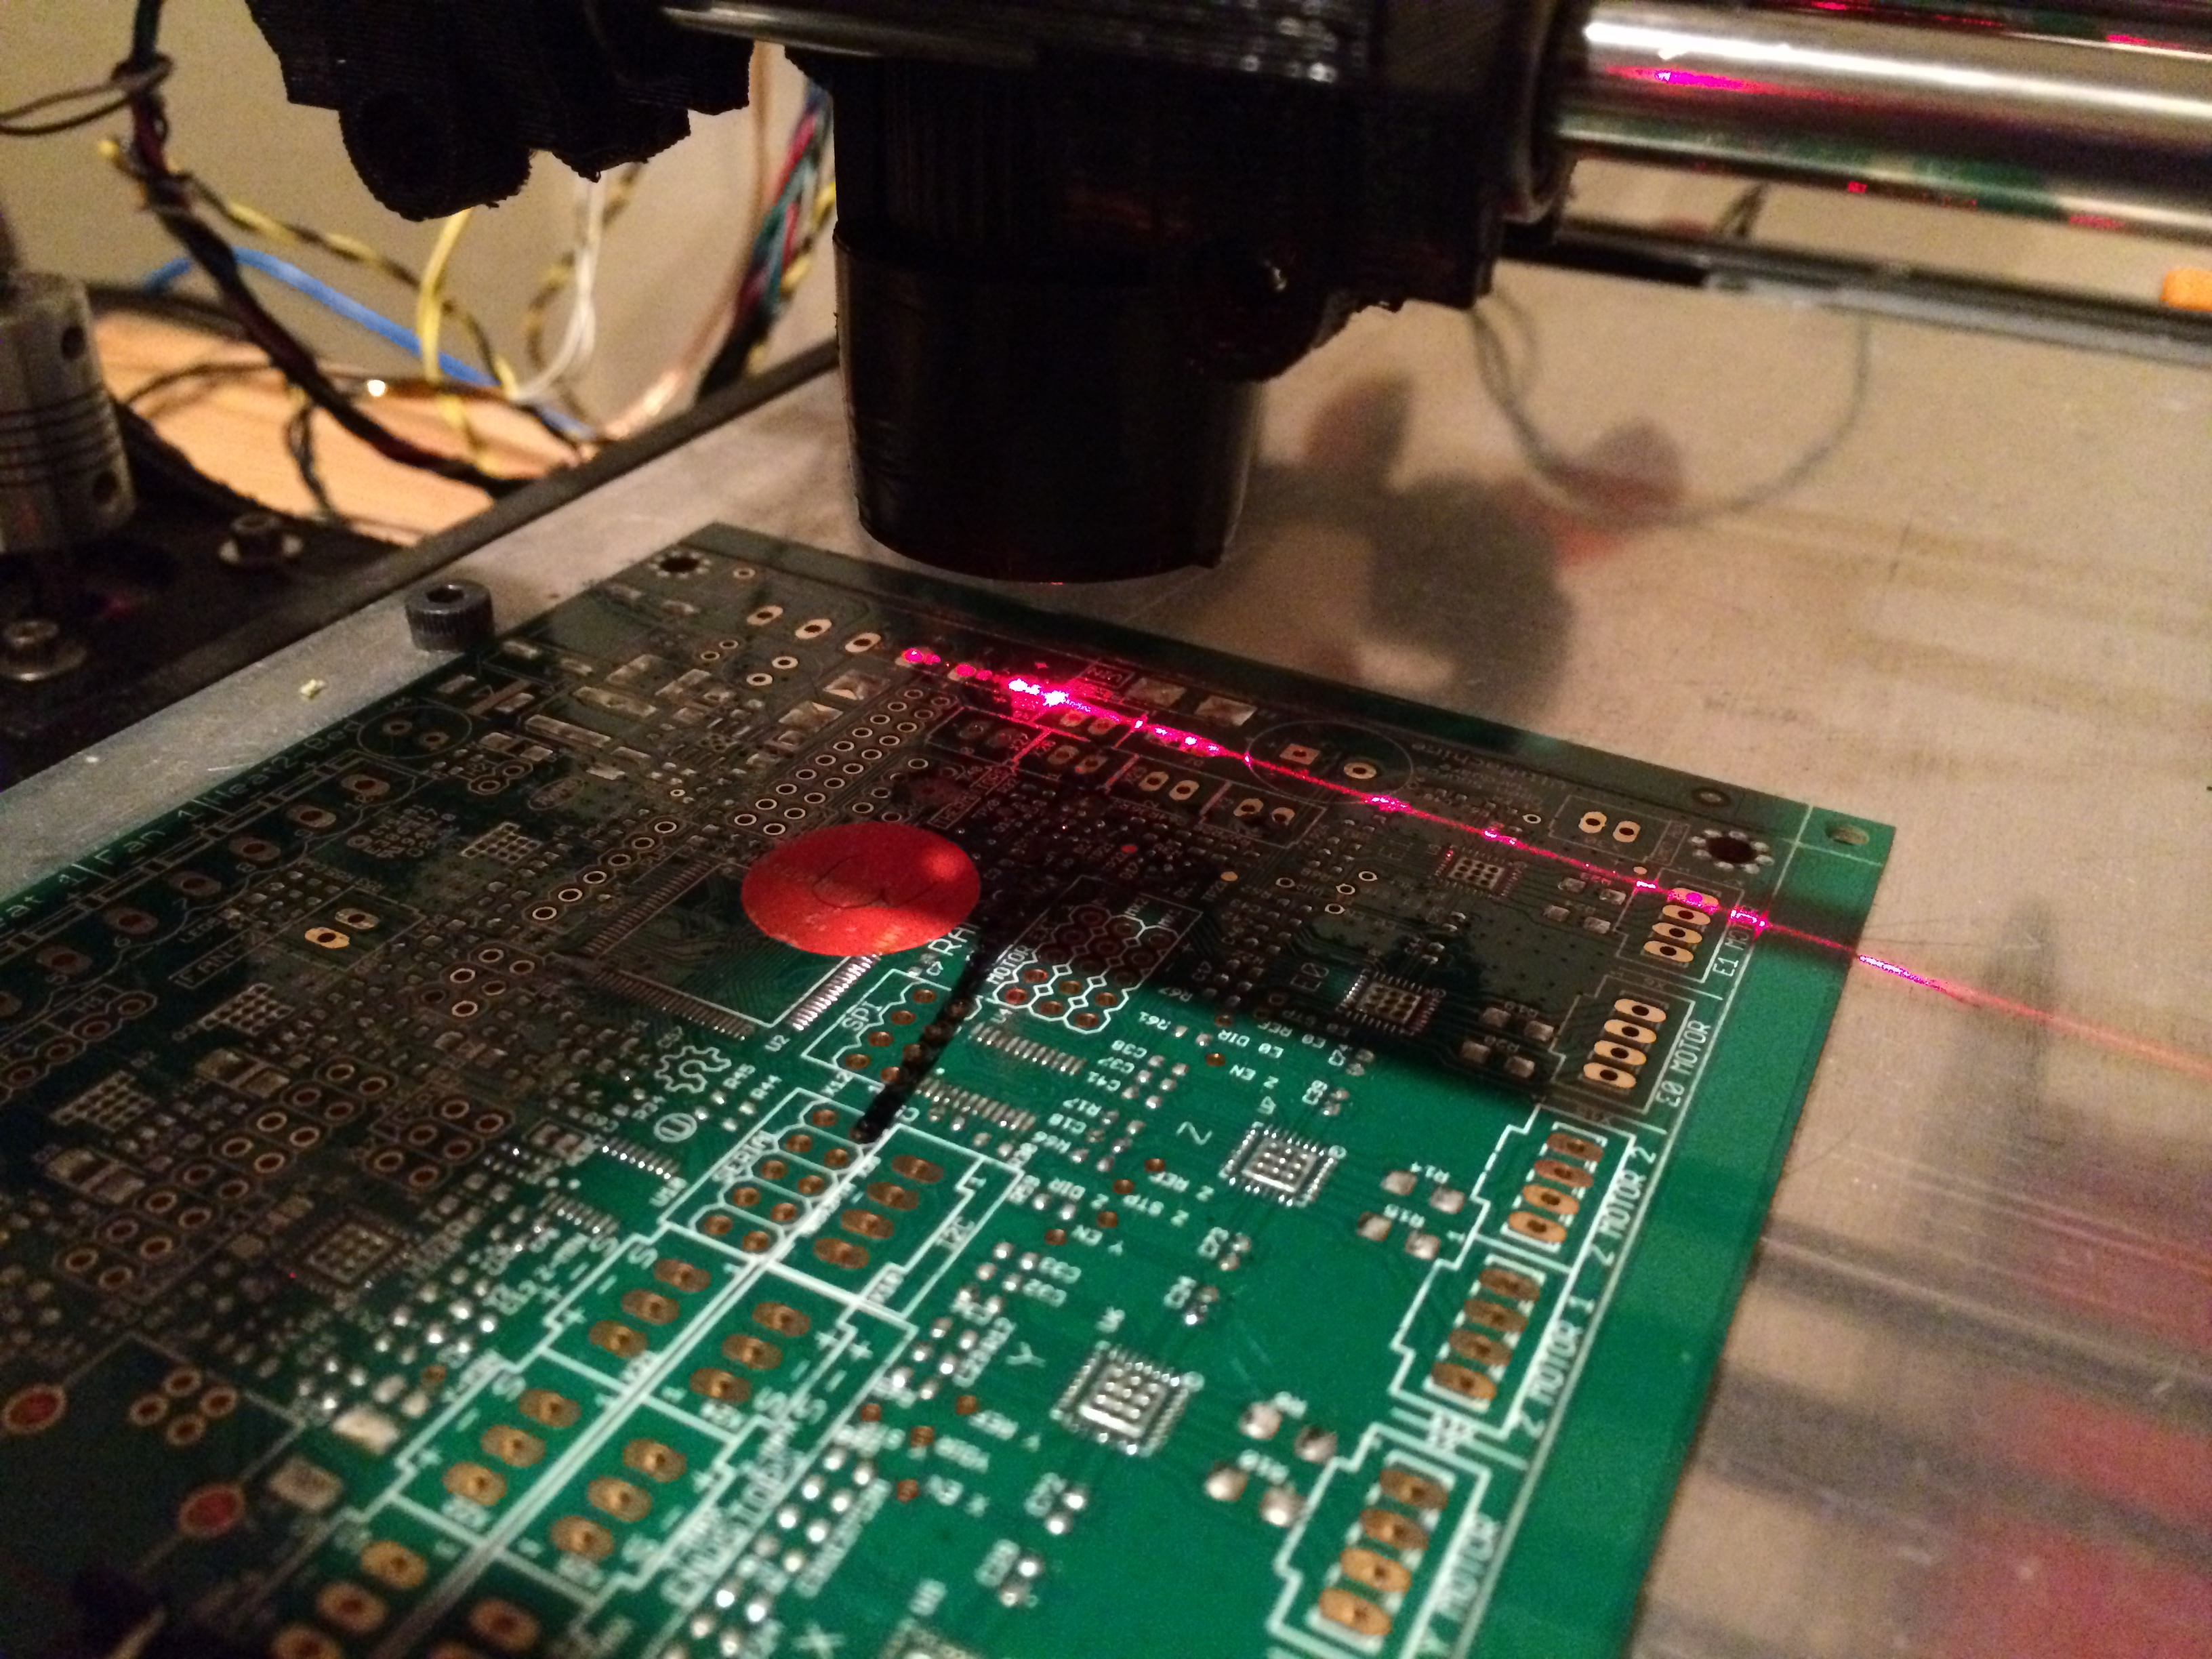
\includegraphics[scale=0.1,angle=270]{images/volume_analysis_setup/IMG_0606.JPG}
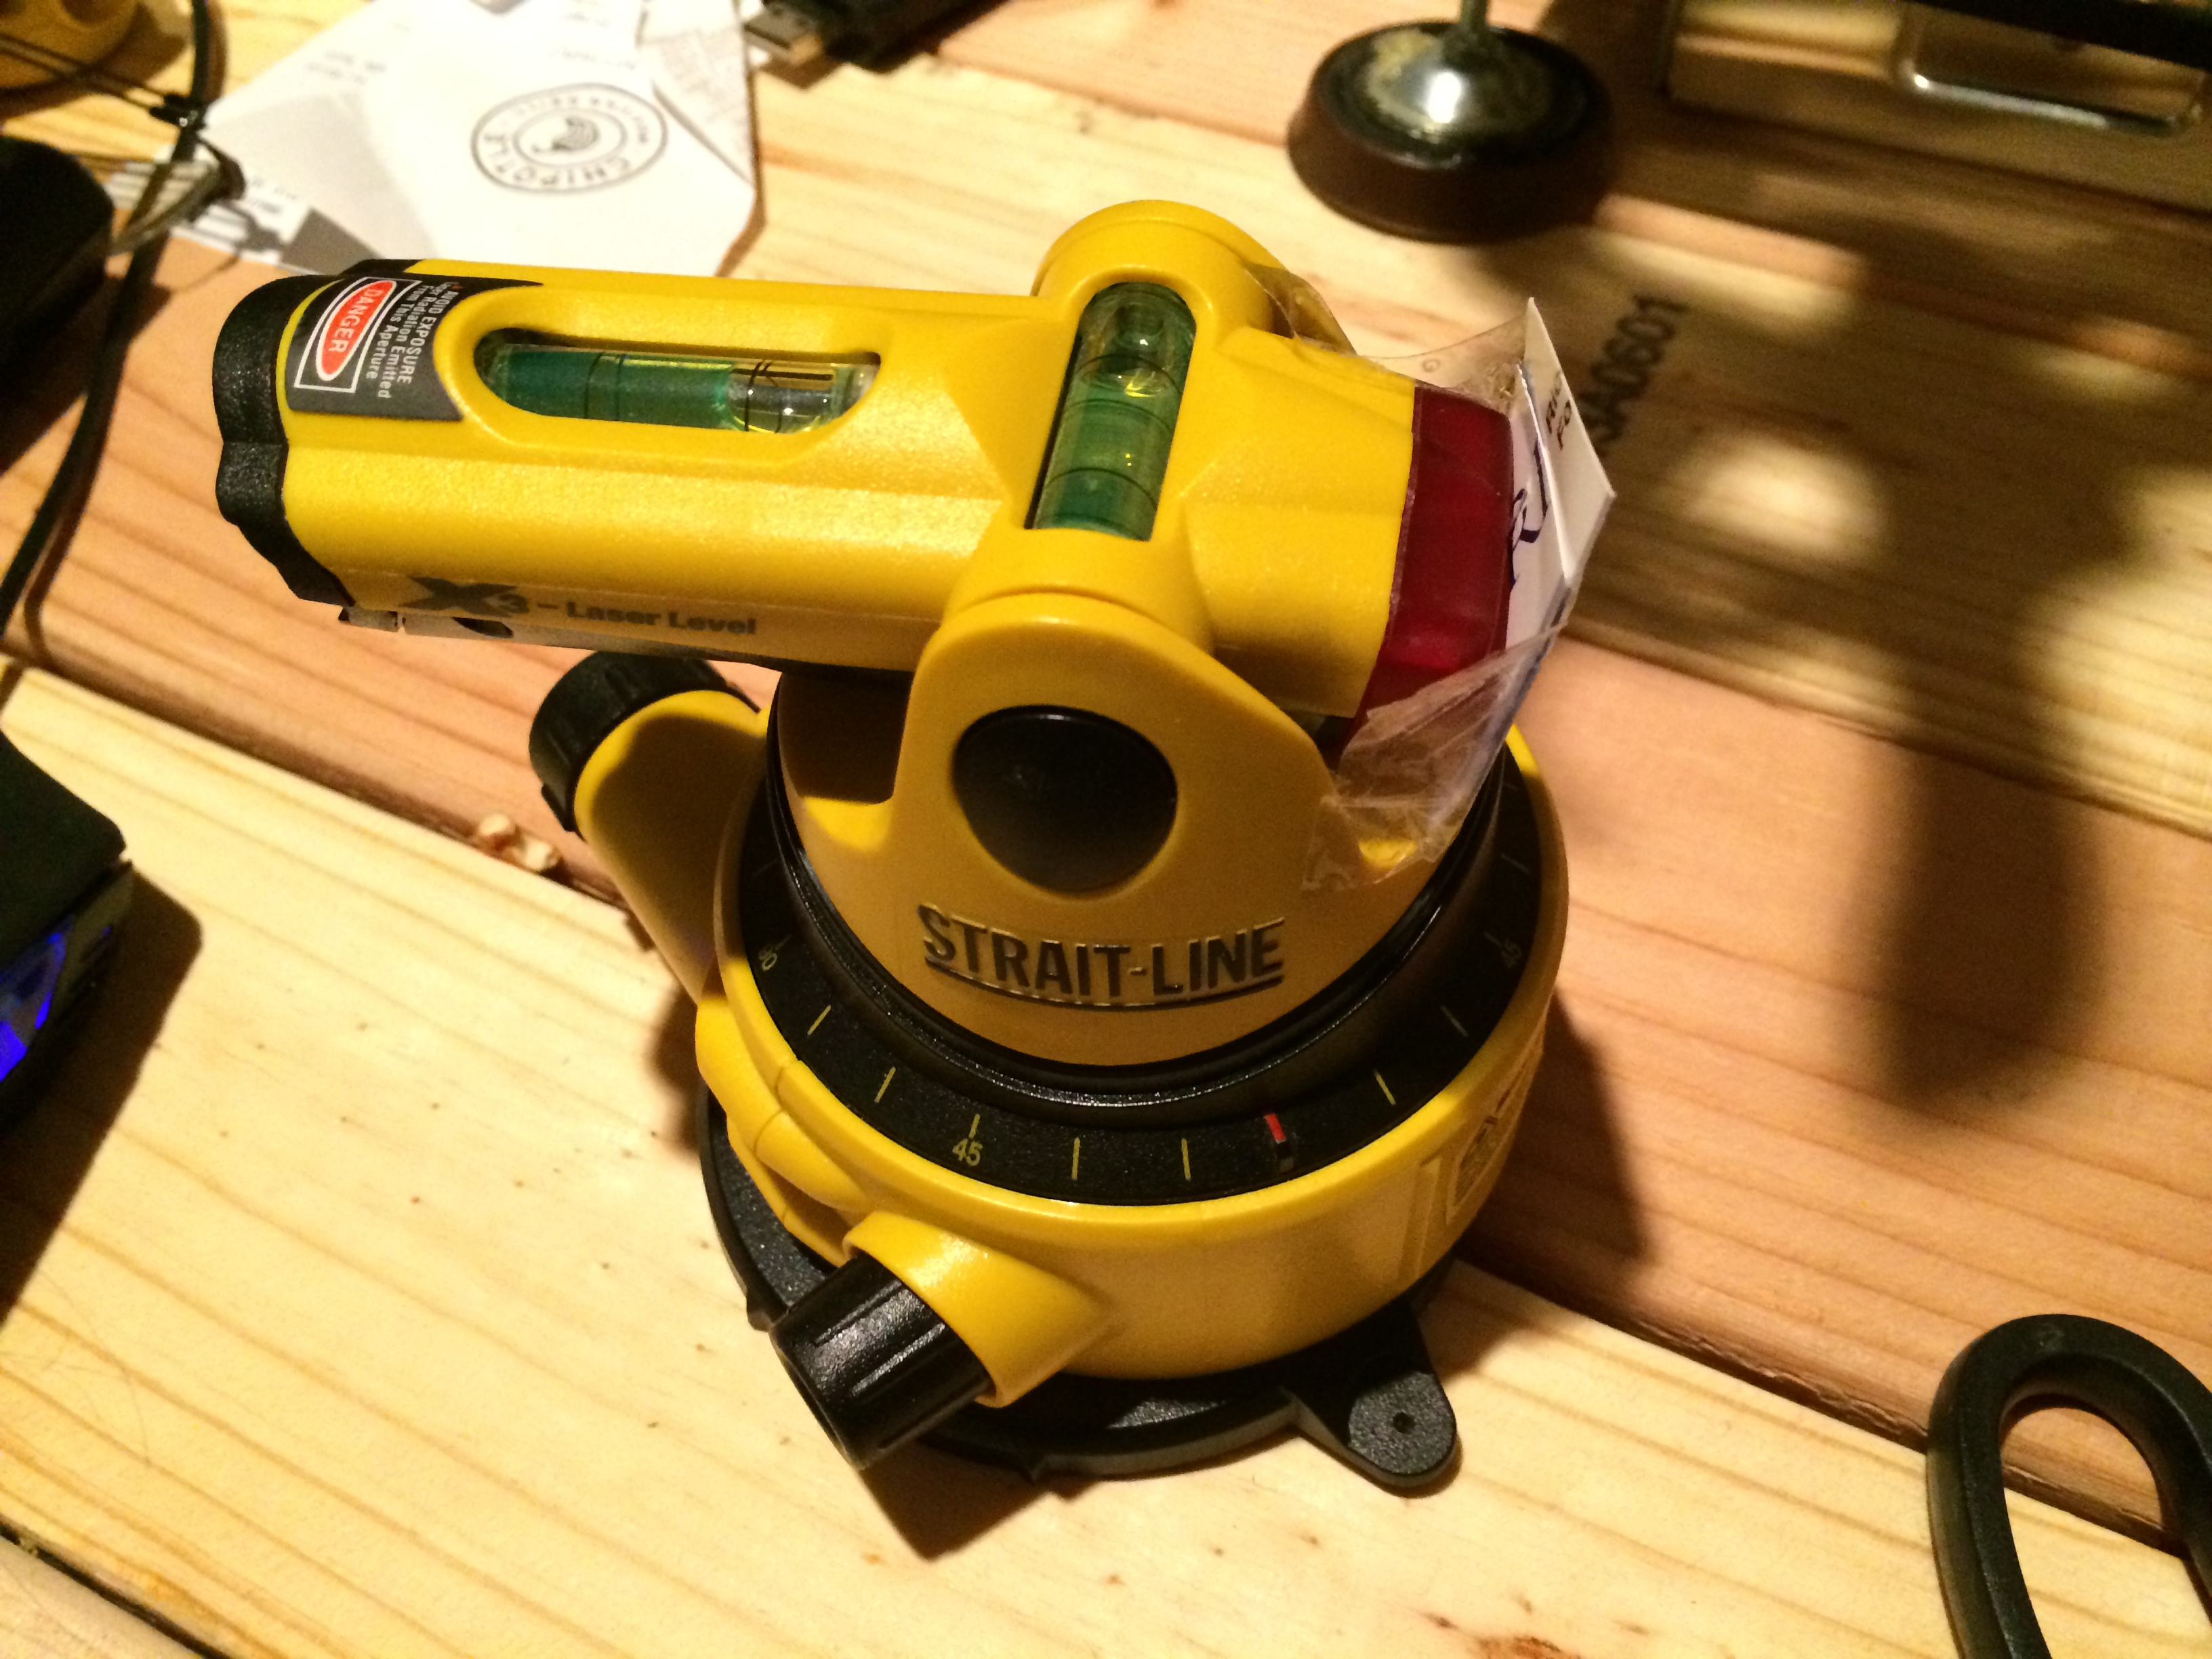
\includegraphics[scale=0.1,angle=270]{images/volume_analysis_setup/IMG_0607.JPG}
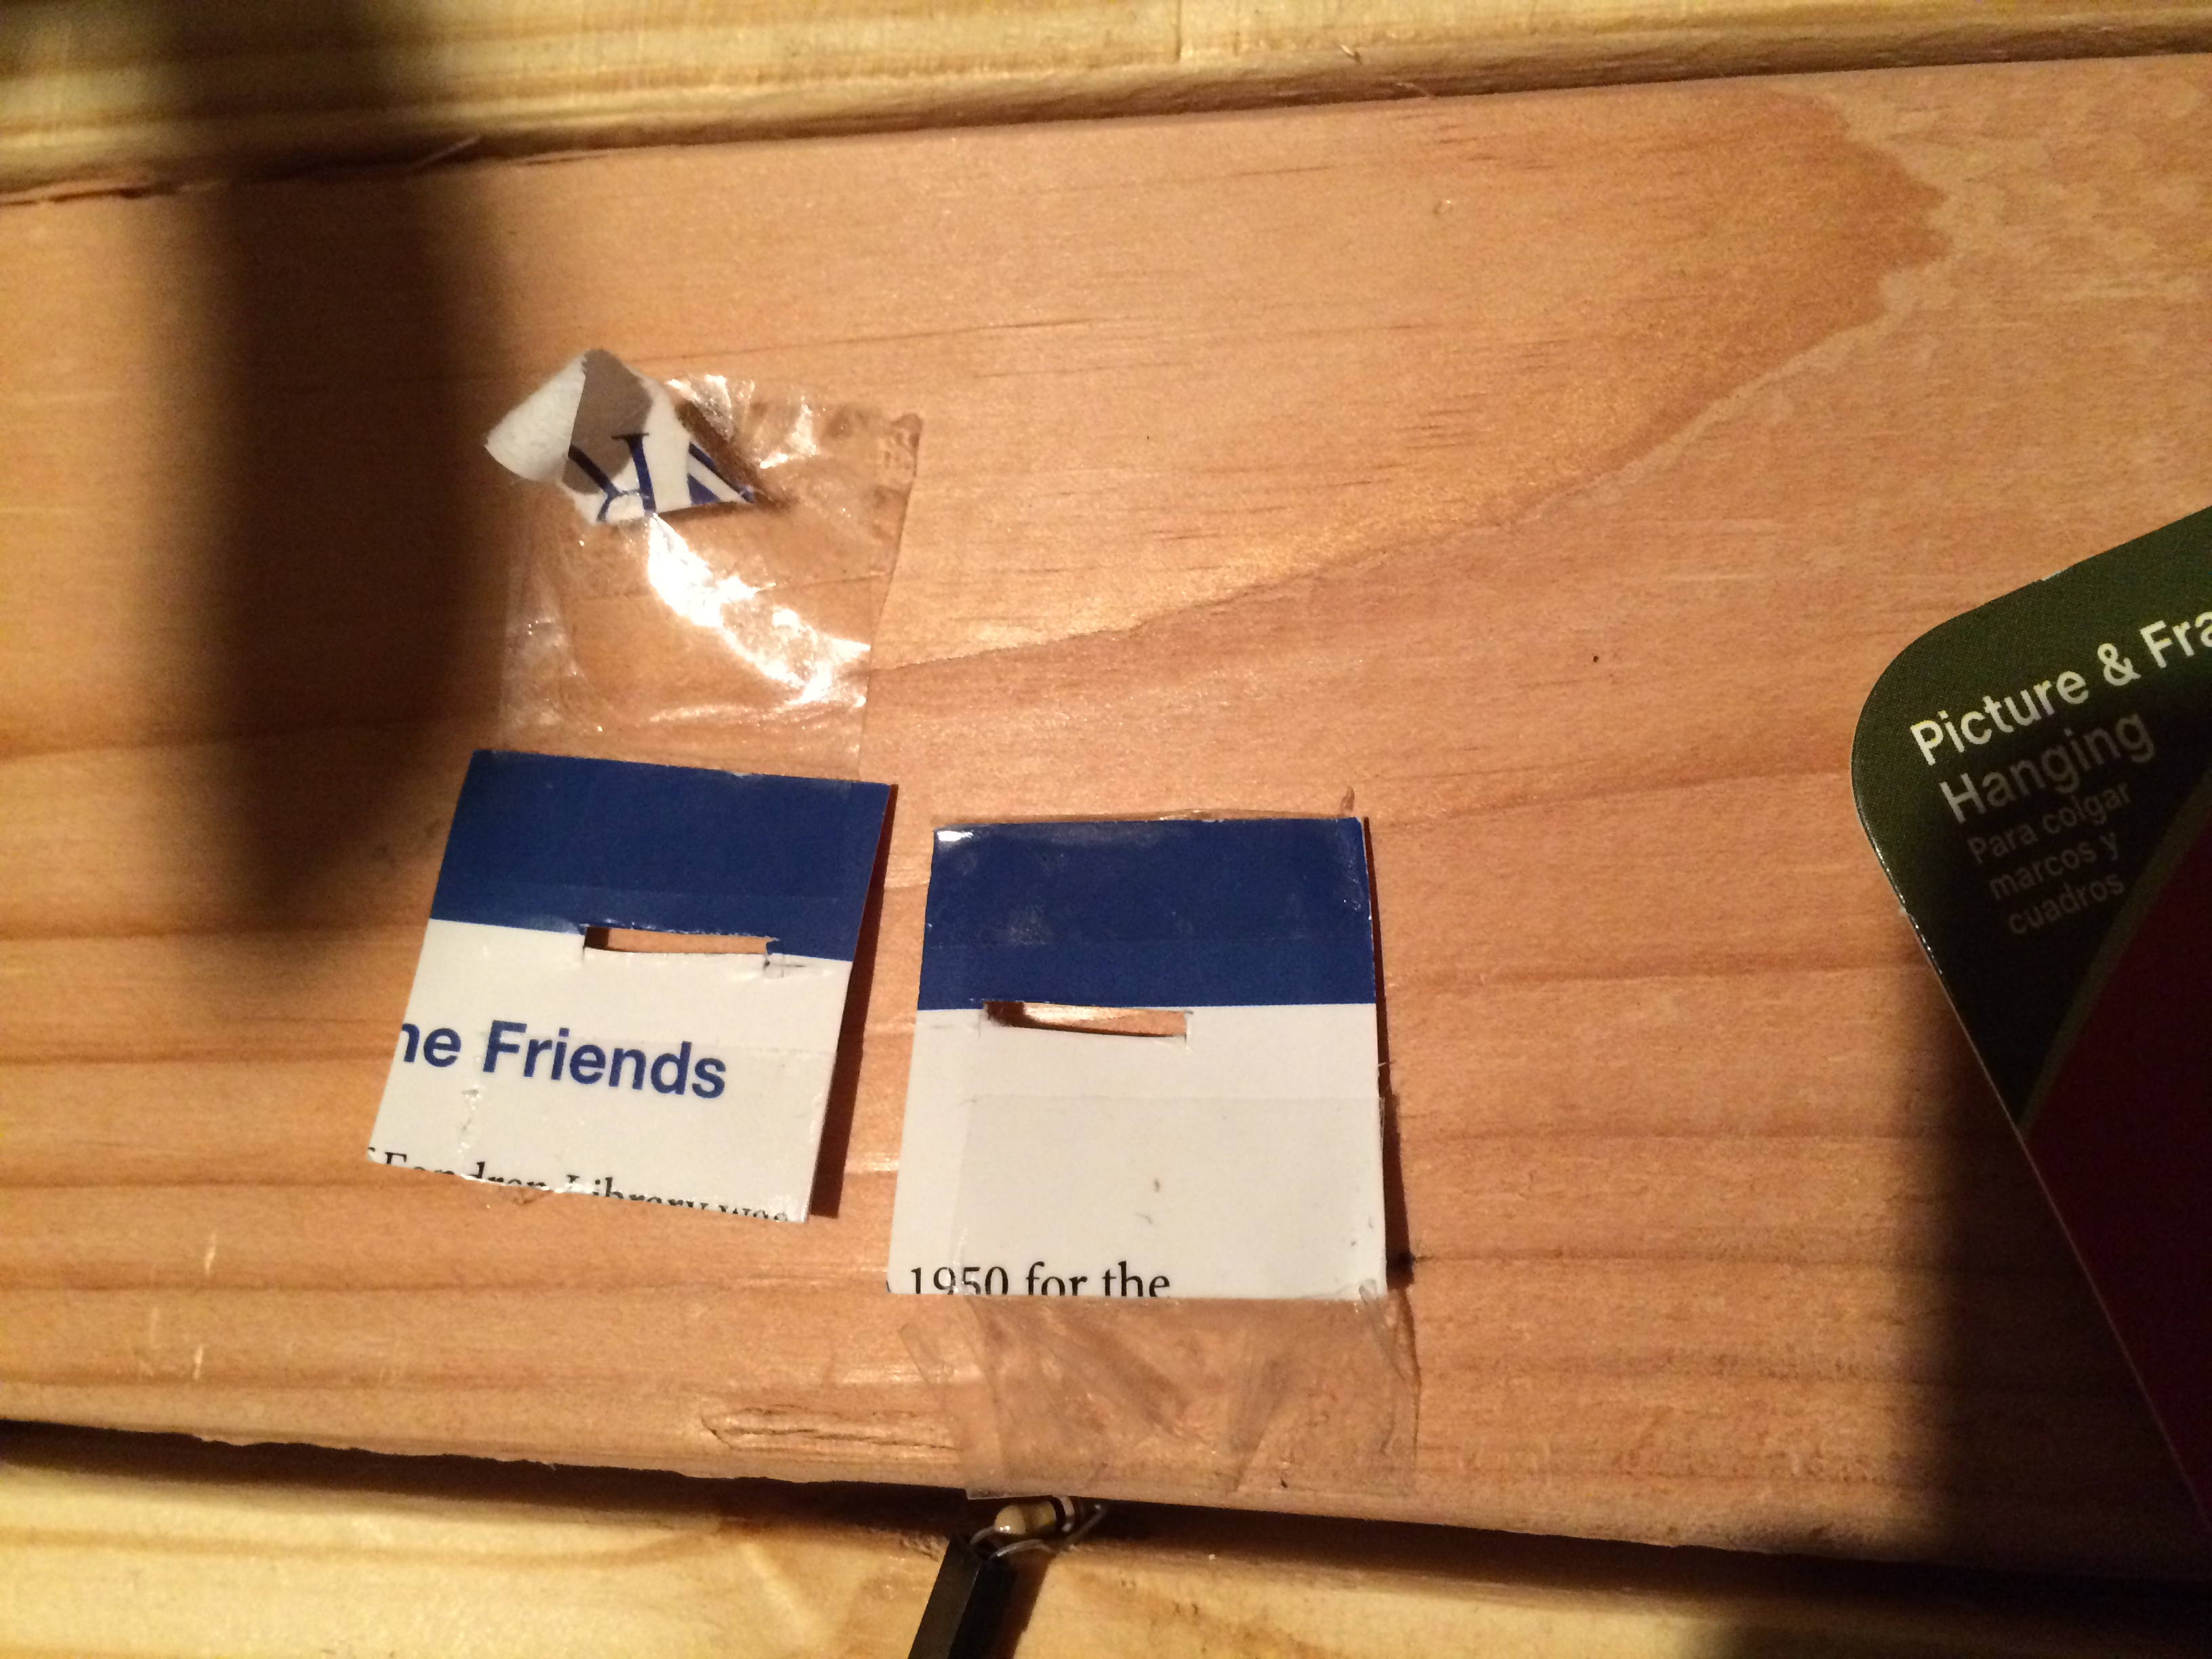
\includegraphics[scale=0.1,angle=270]{images/volume_analysis_setup/IMG_0608.JPG}
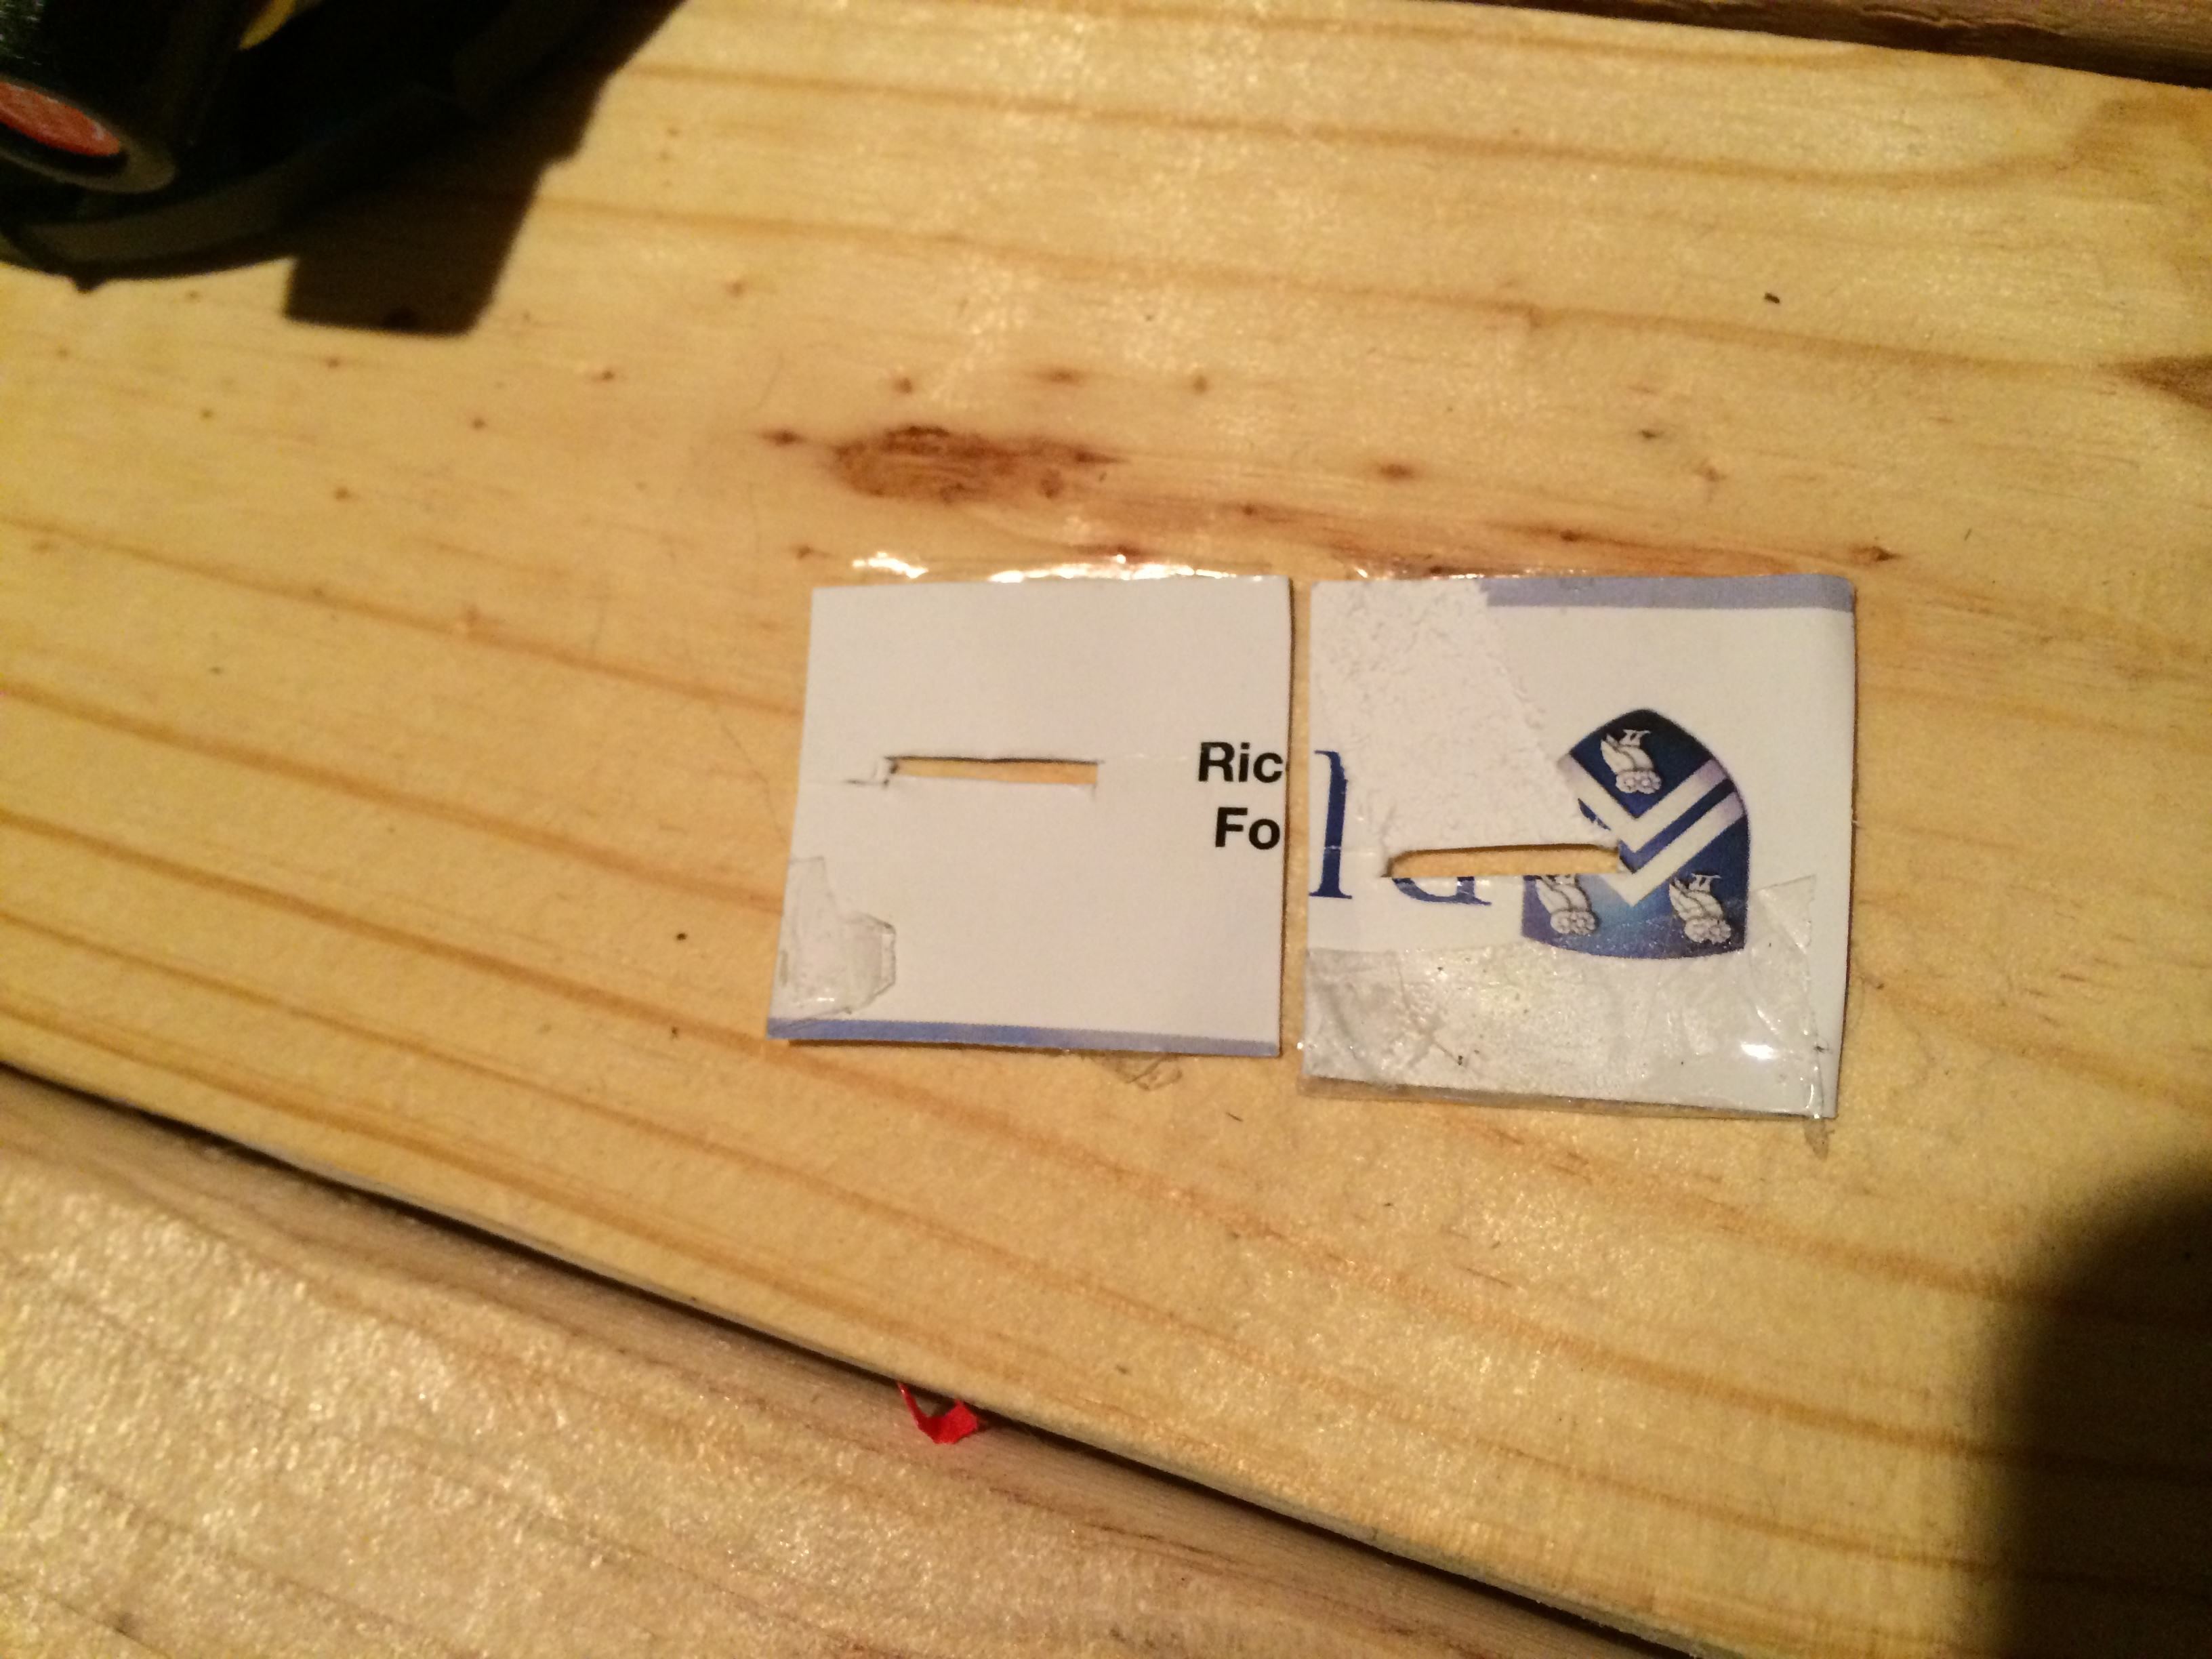
\includegraphics[scale=0.1,angle=270]{images/volume_analysis_setup/IMG_0609.JPG}
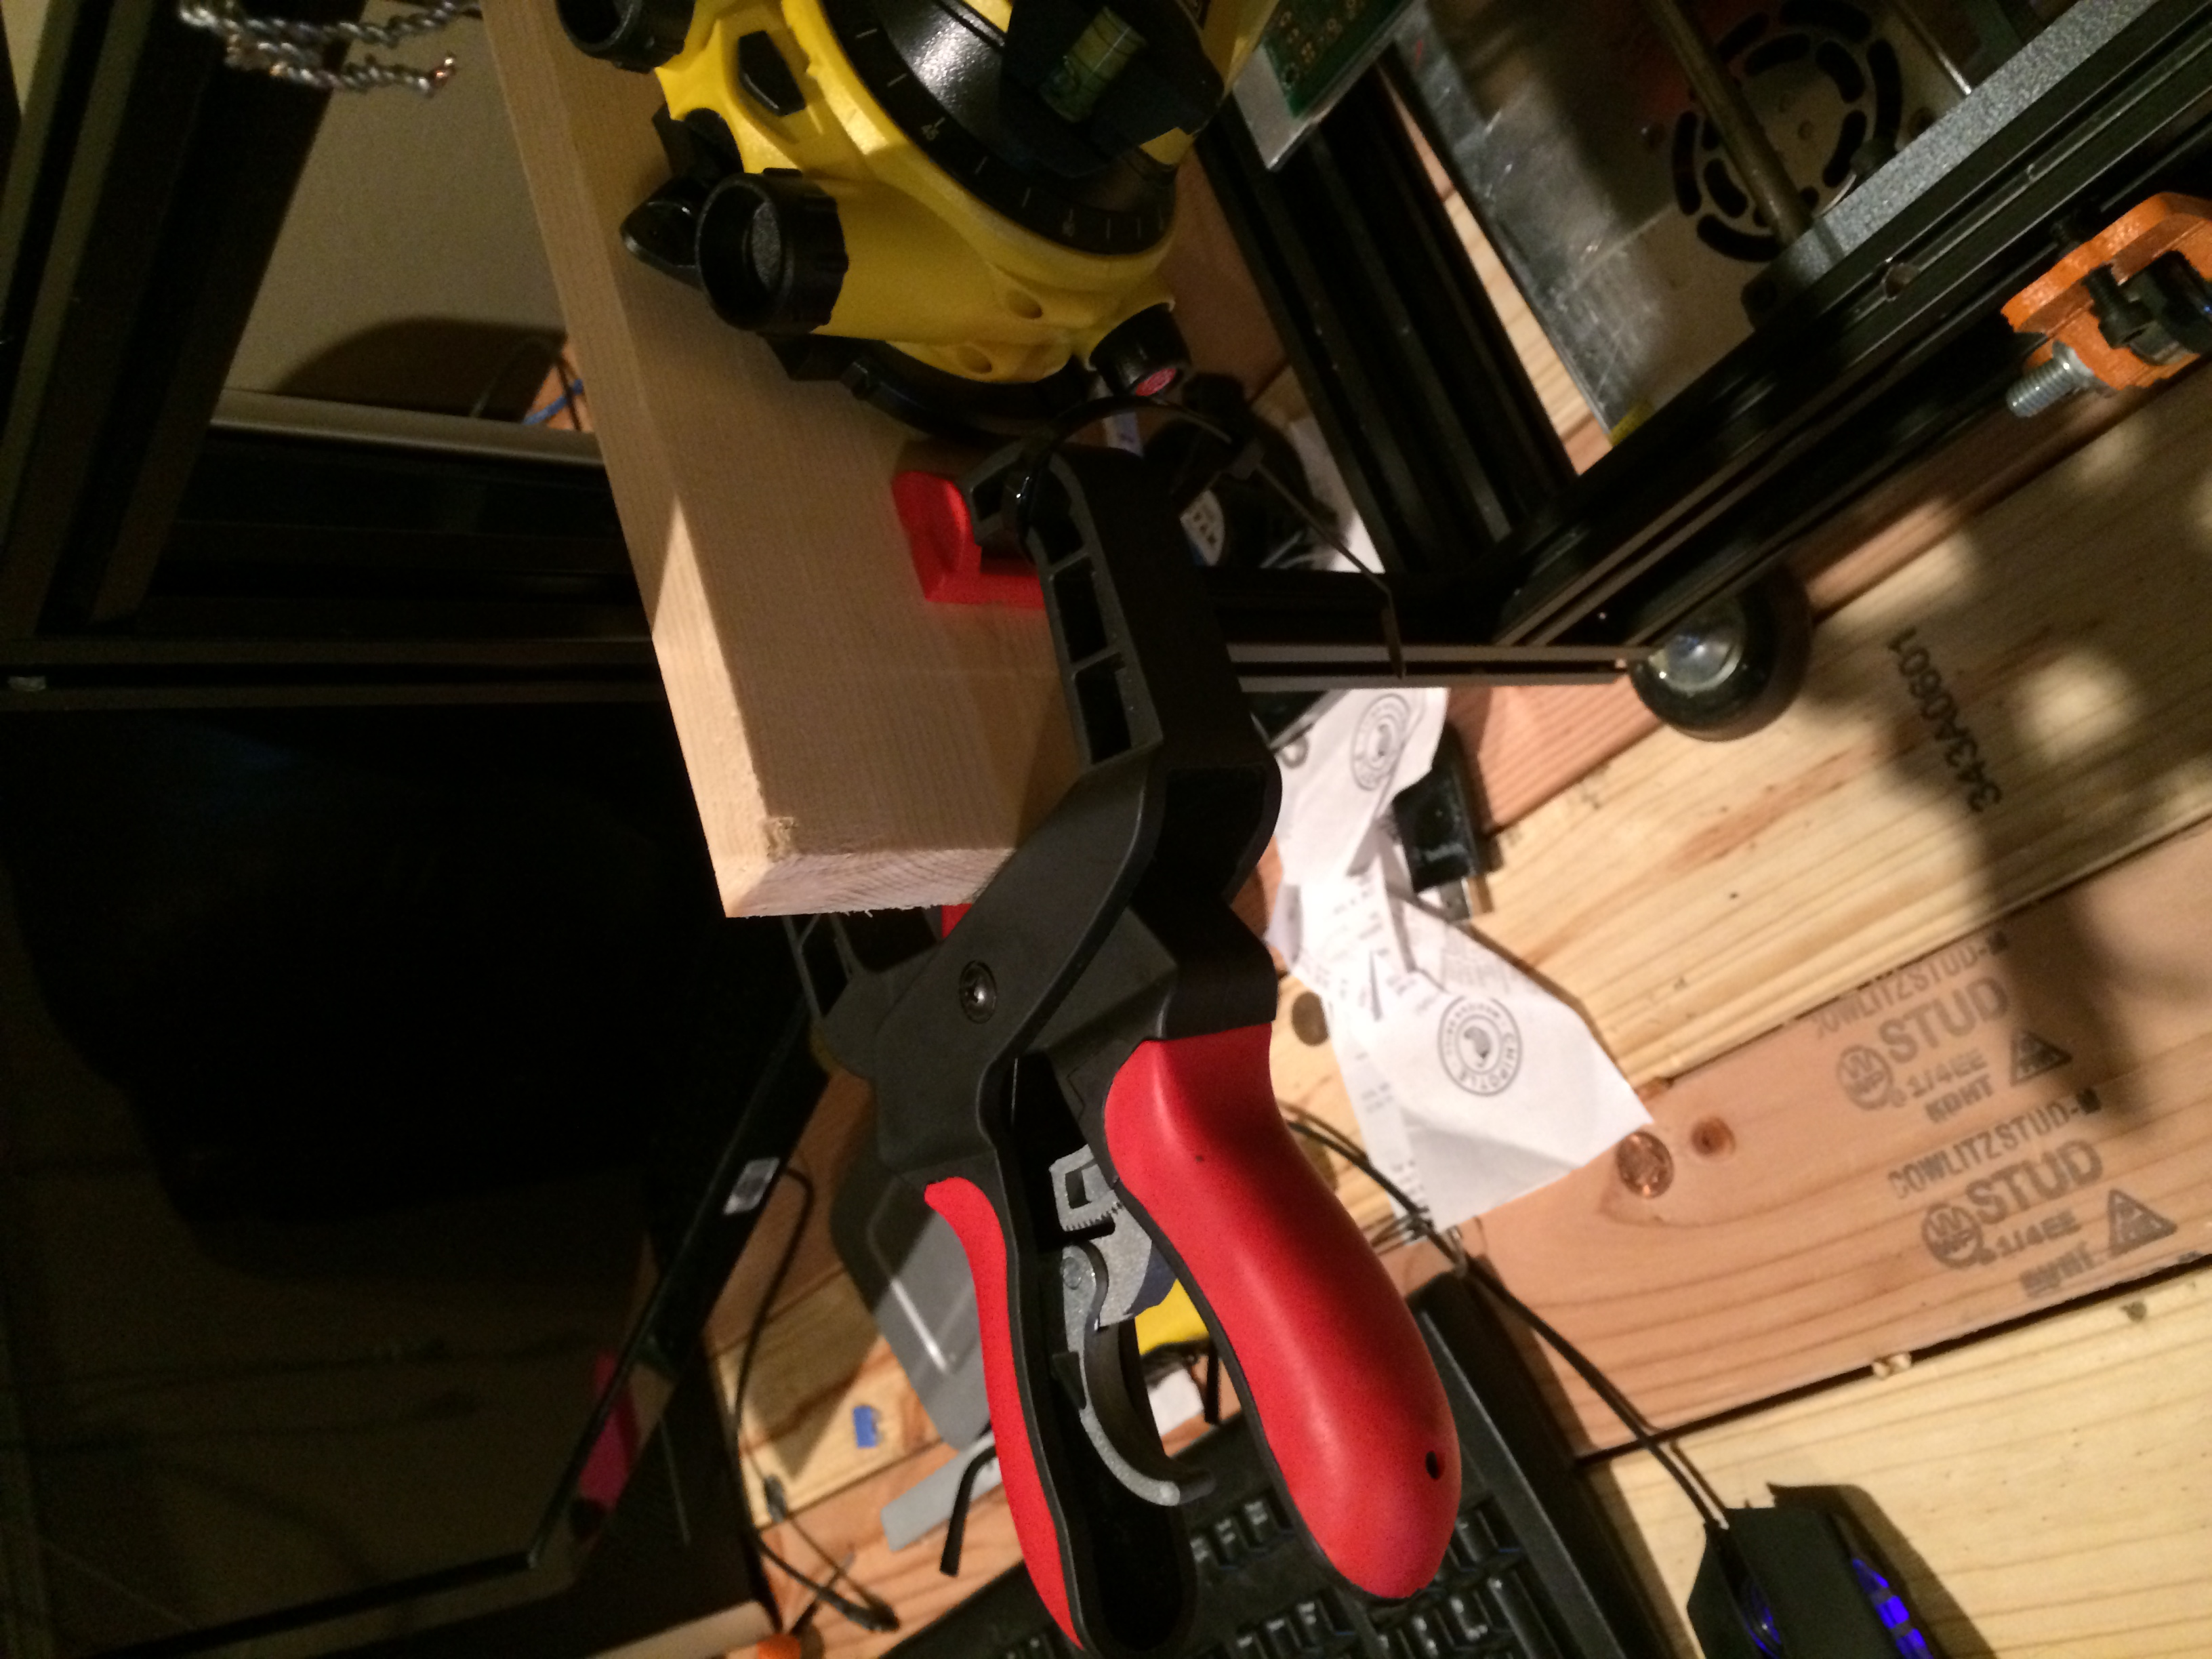
\includegraphics[scale=0.1,angle=270]{images/volume_analysis_setup/IMG_0610.JPG}
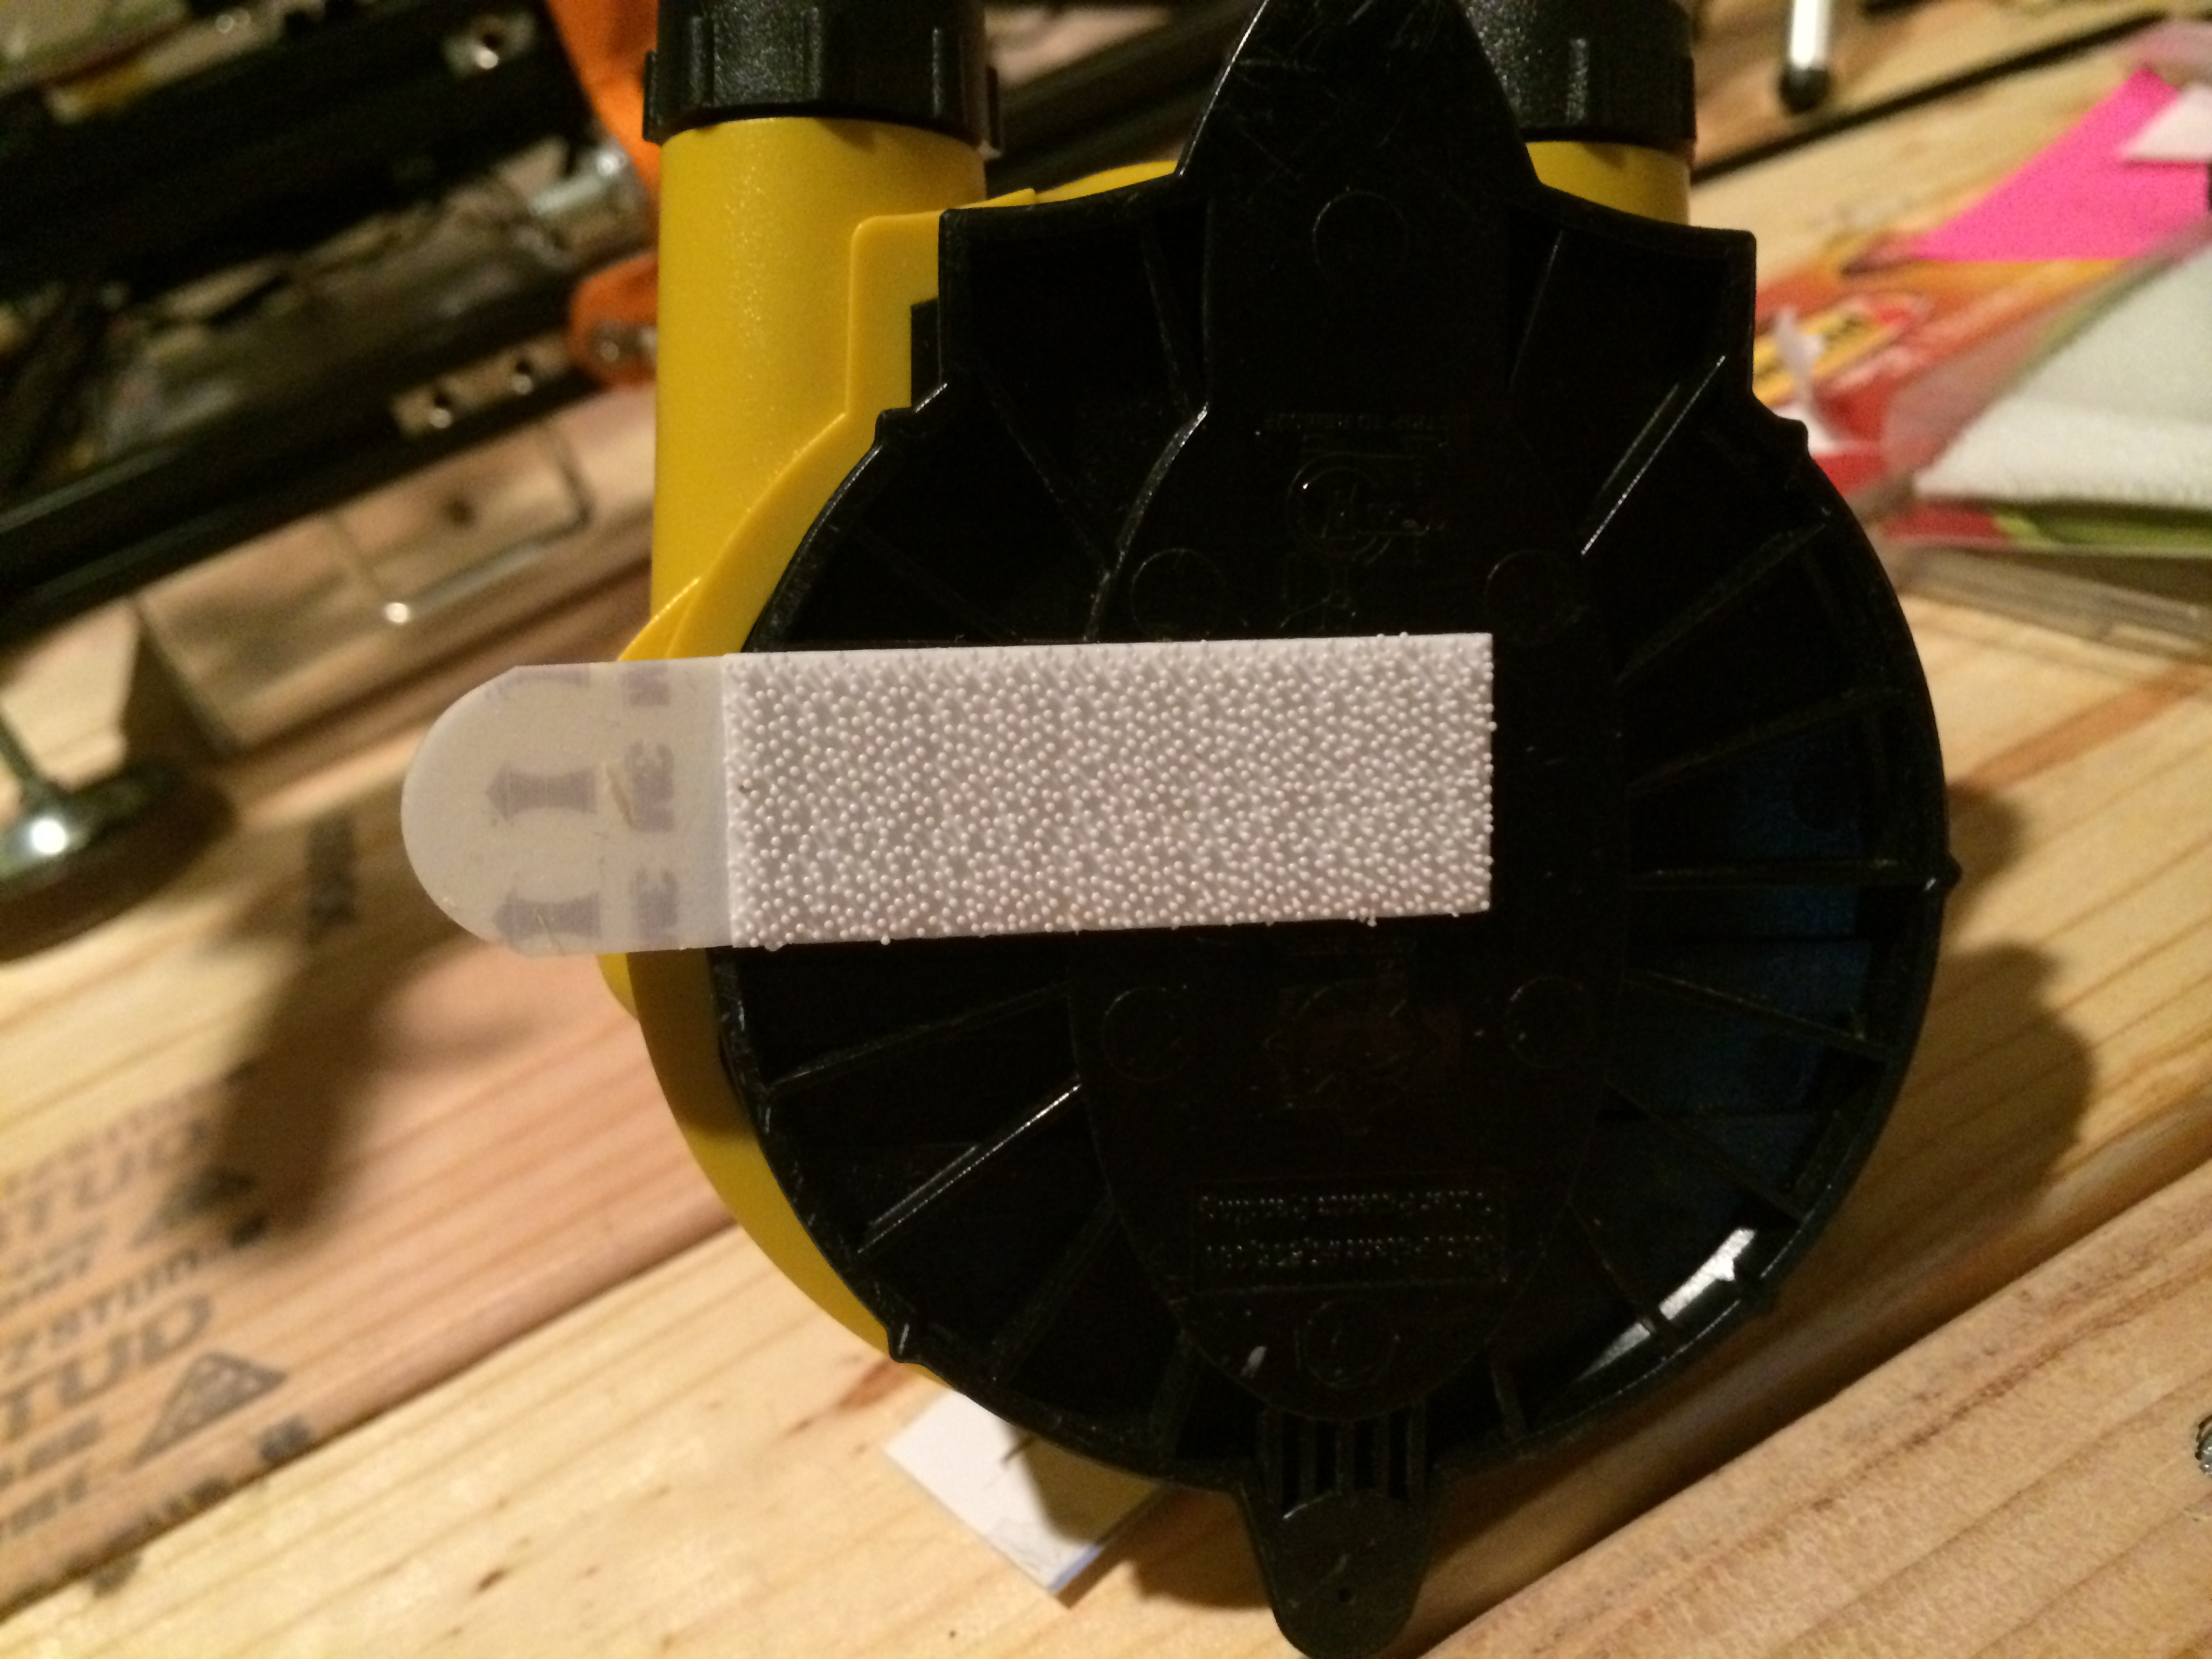
\includegraphics[scale=0.1,angle=270]{images/volume_analysis_setup/IMG_0611.JPG}
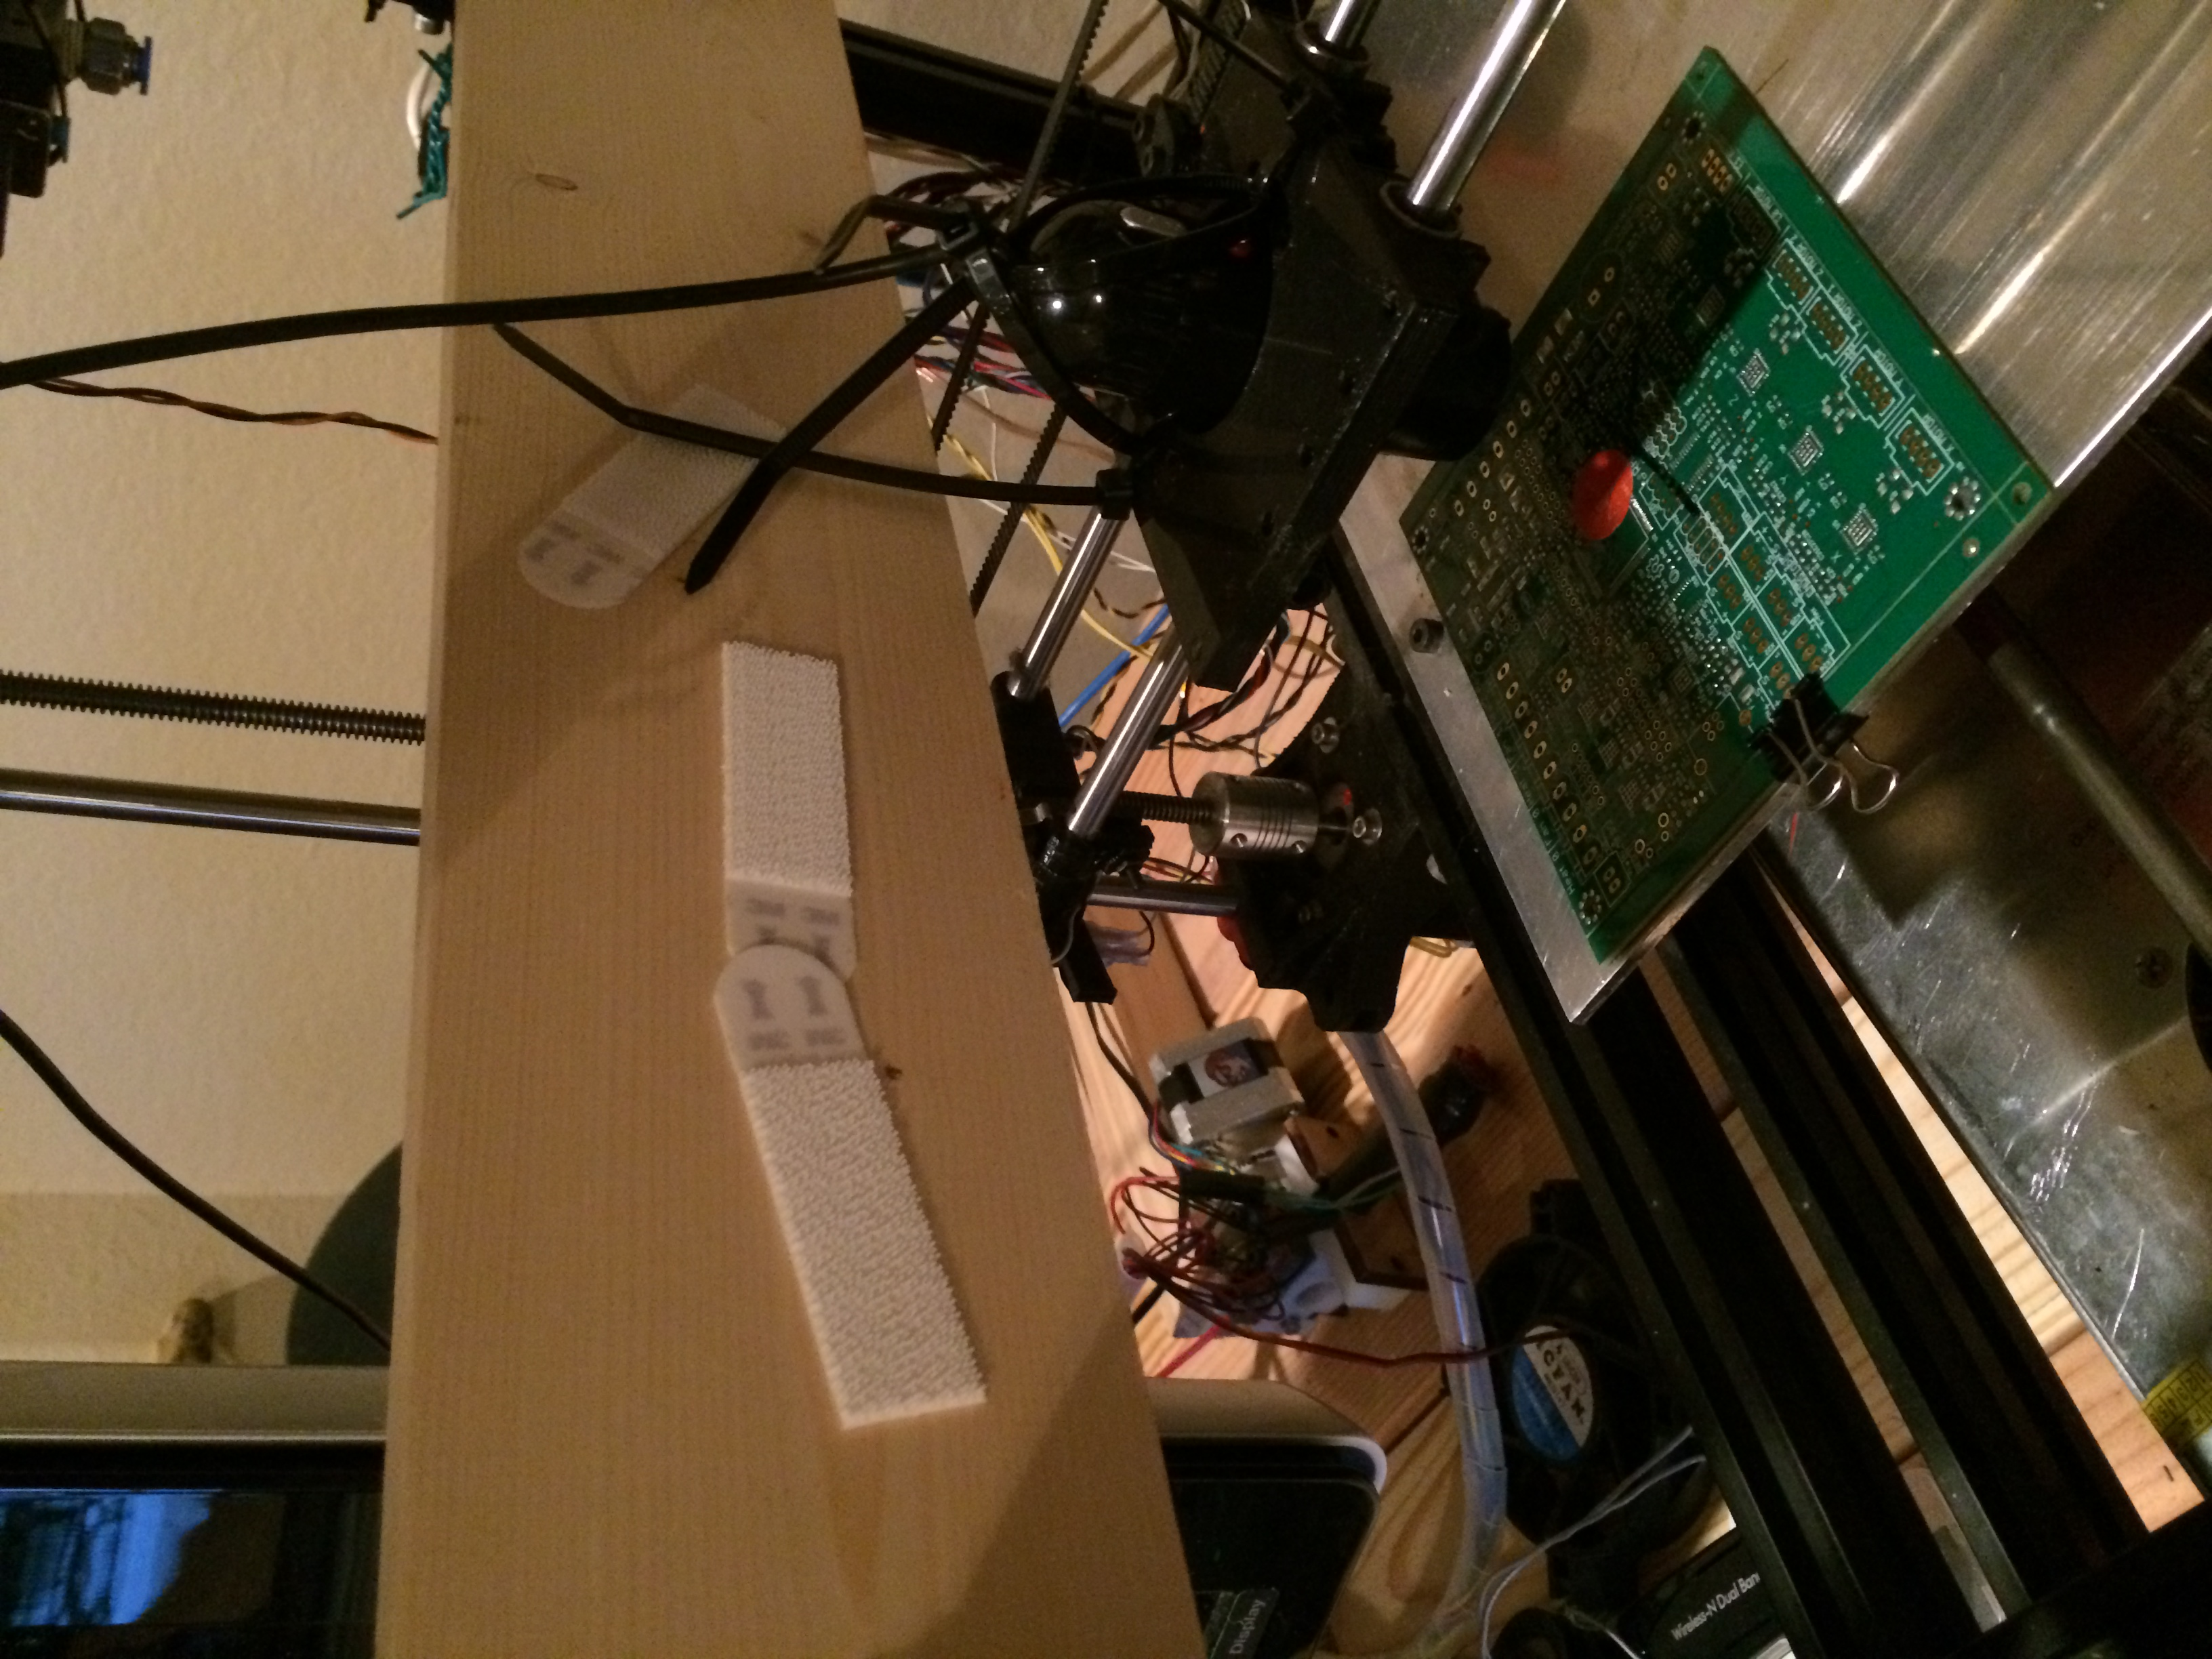
\includegraphics[scale=0.1,angle=270]{images/volume_analysis_setup/IMG_0612.JPG}
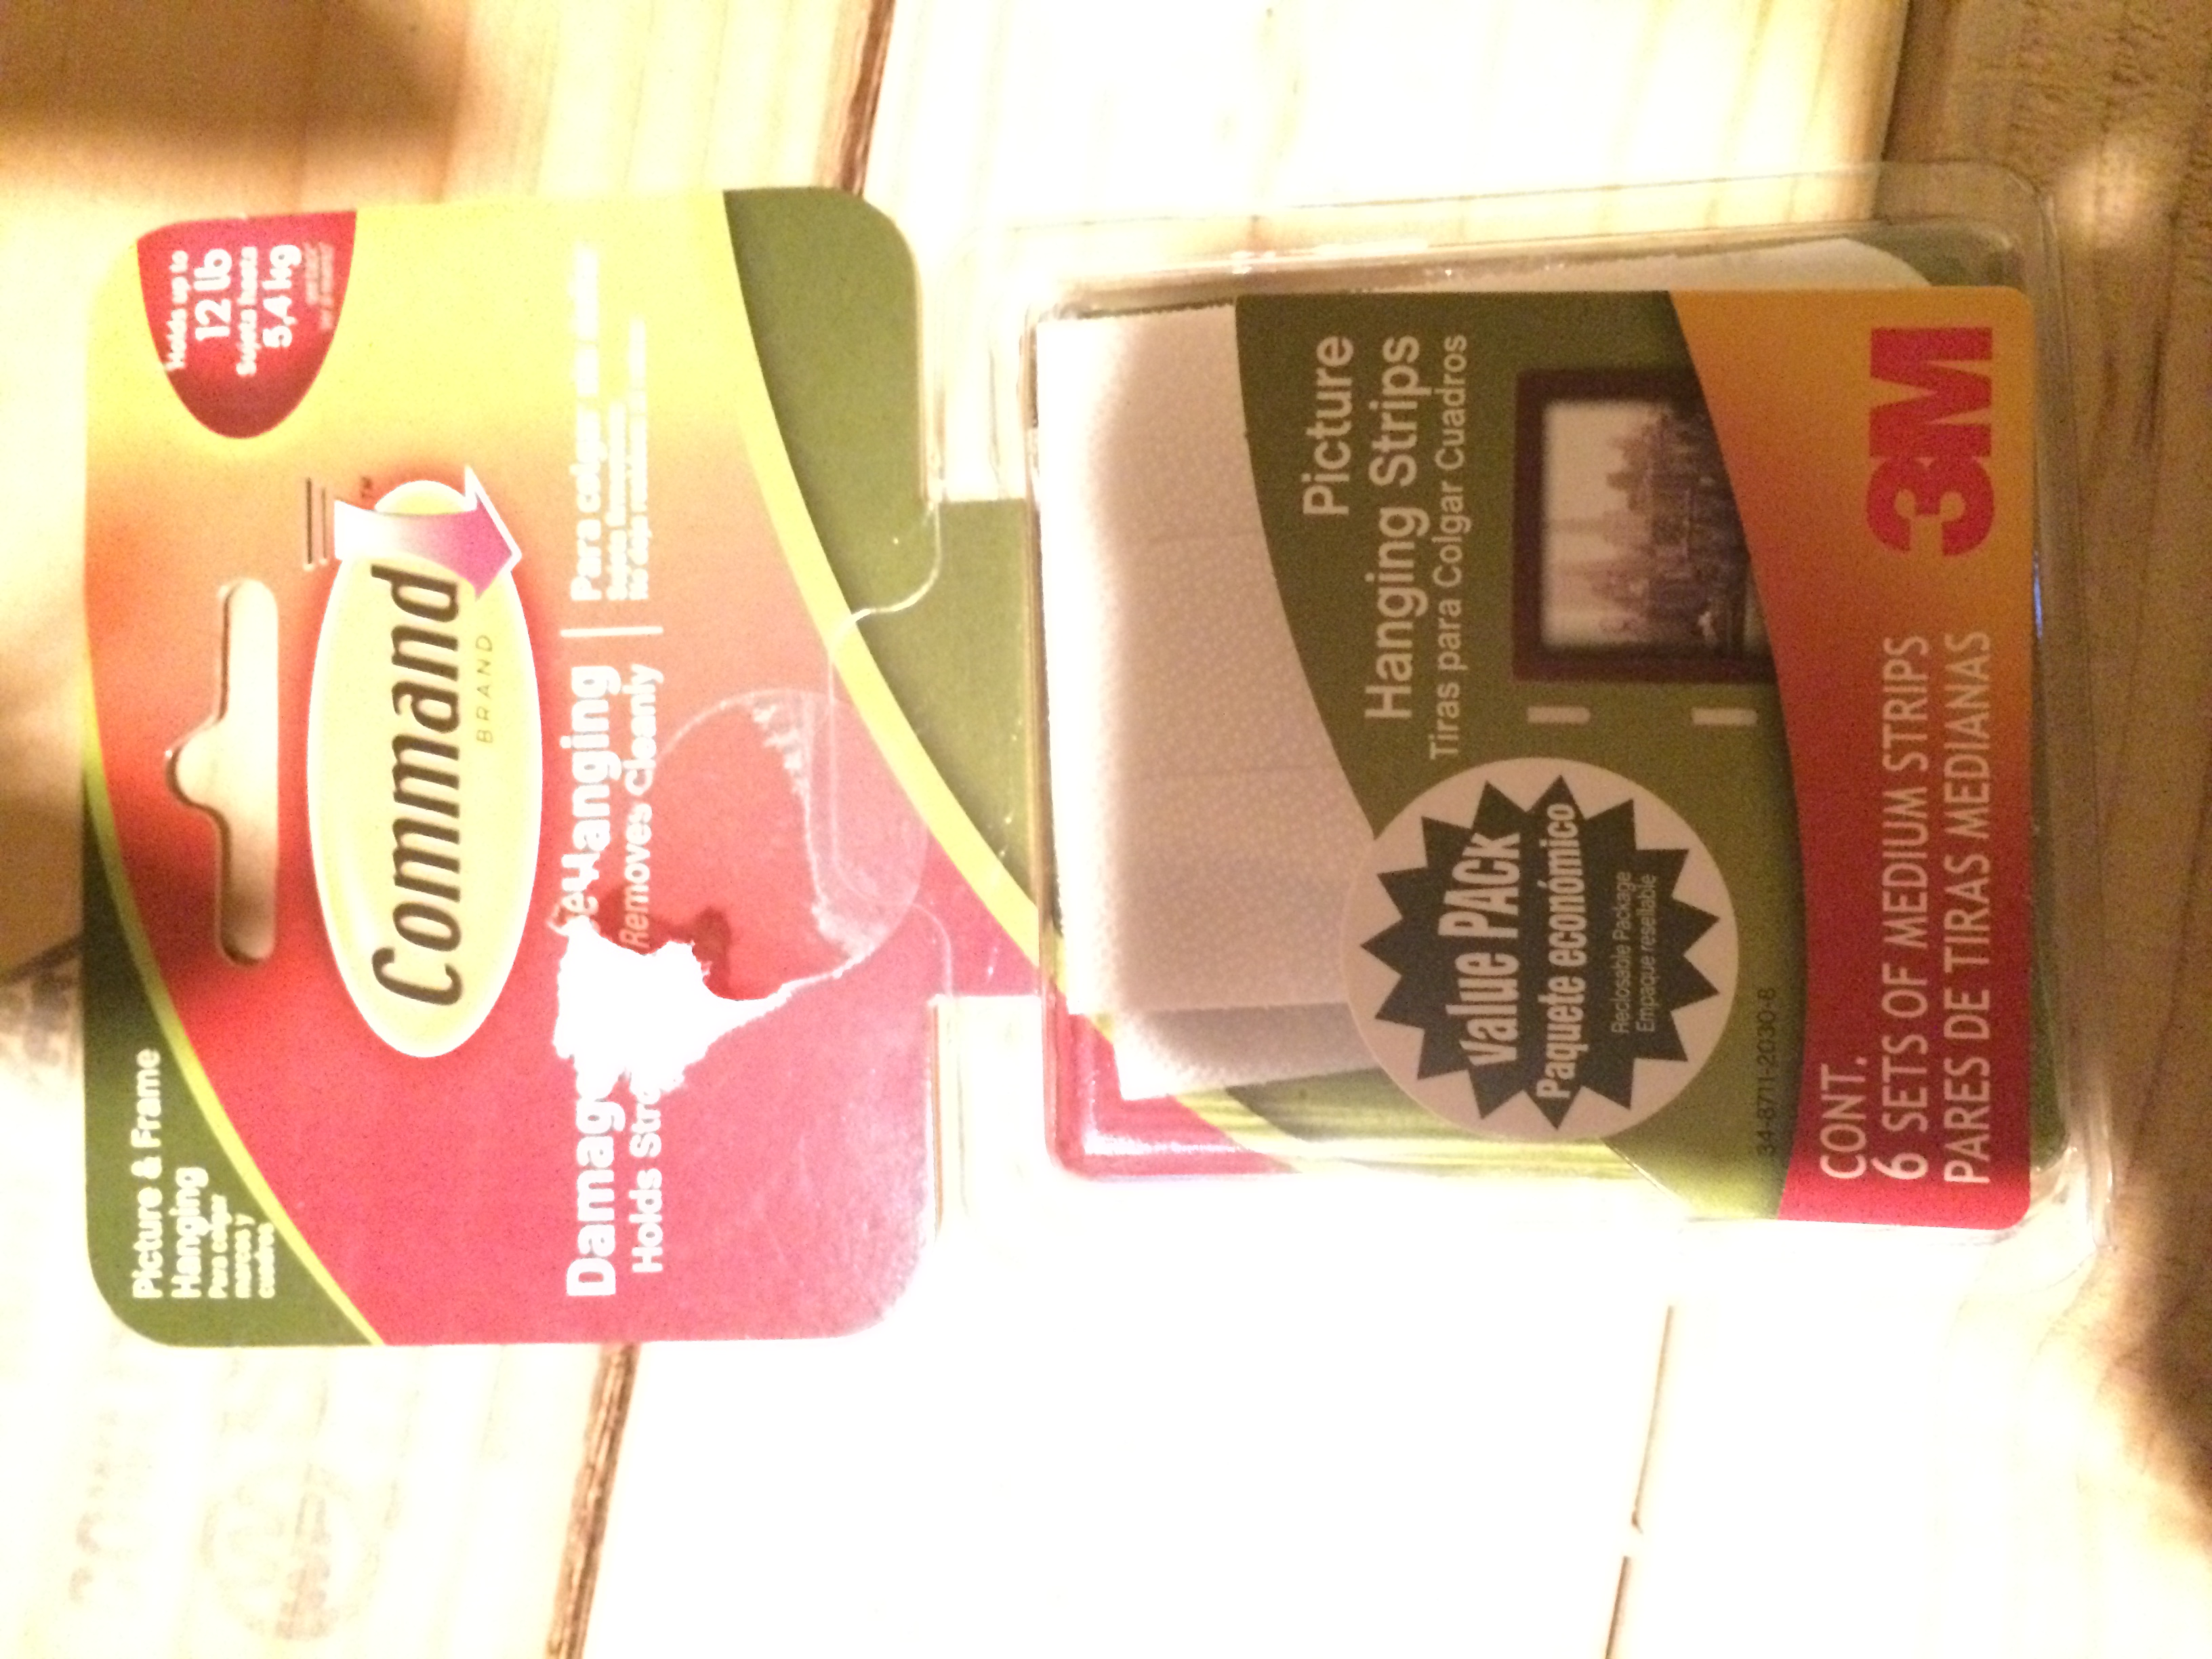
\includegraphics[scale=0.1,angle=270]{images/volume_analysis_setup/IMG_0613.JPG}
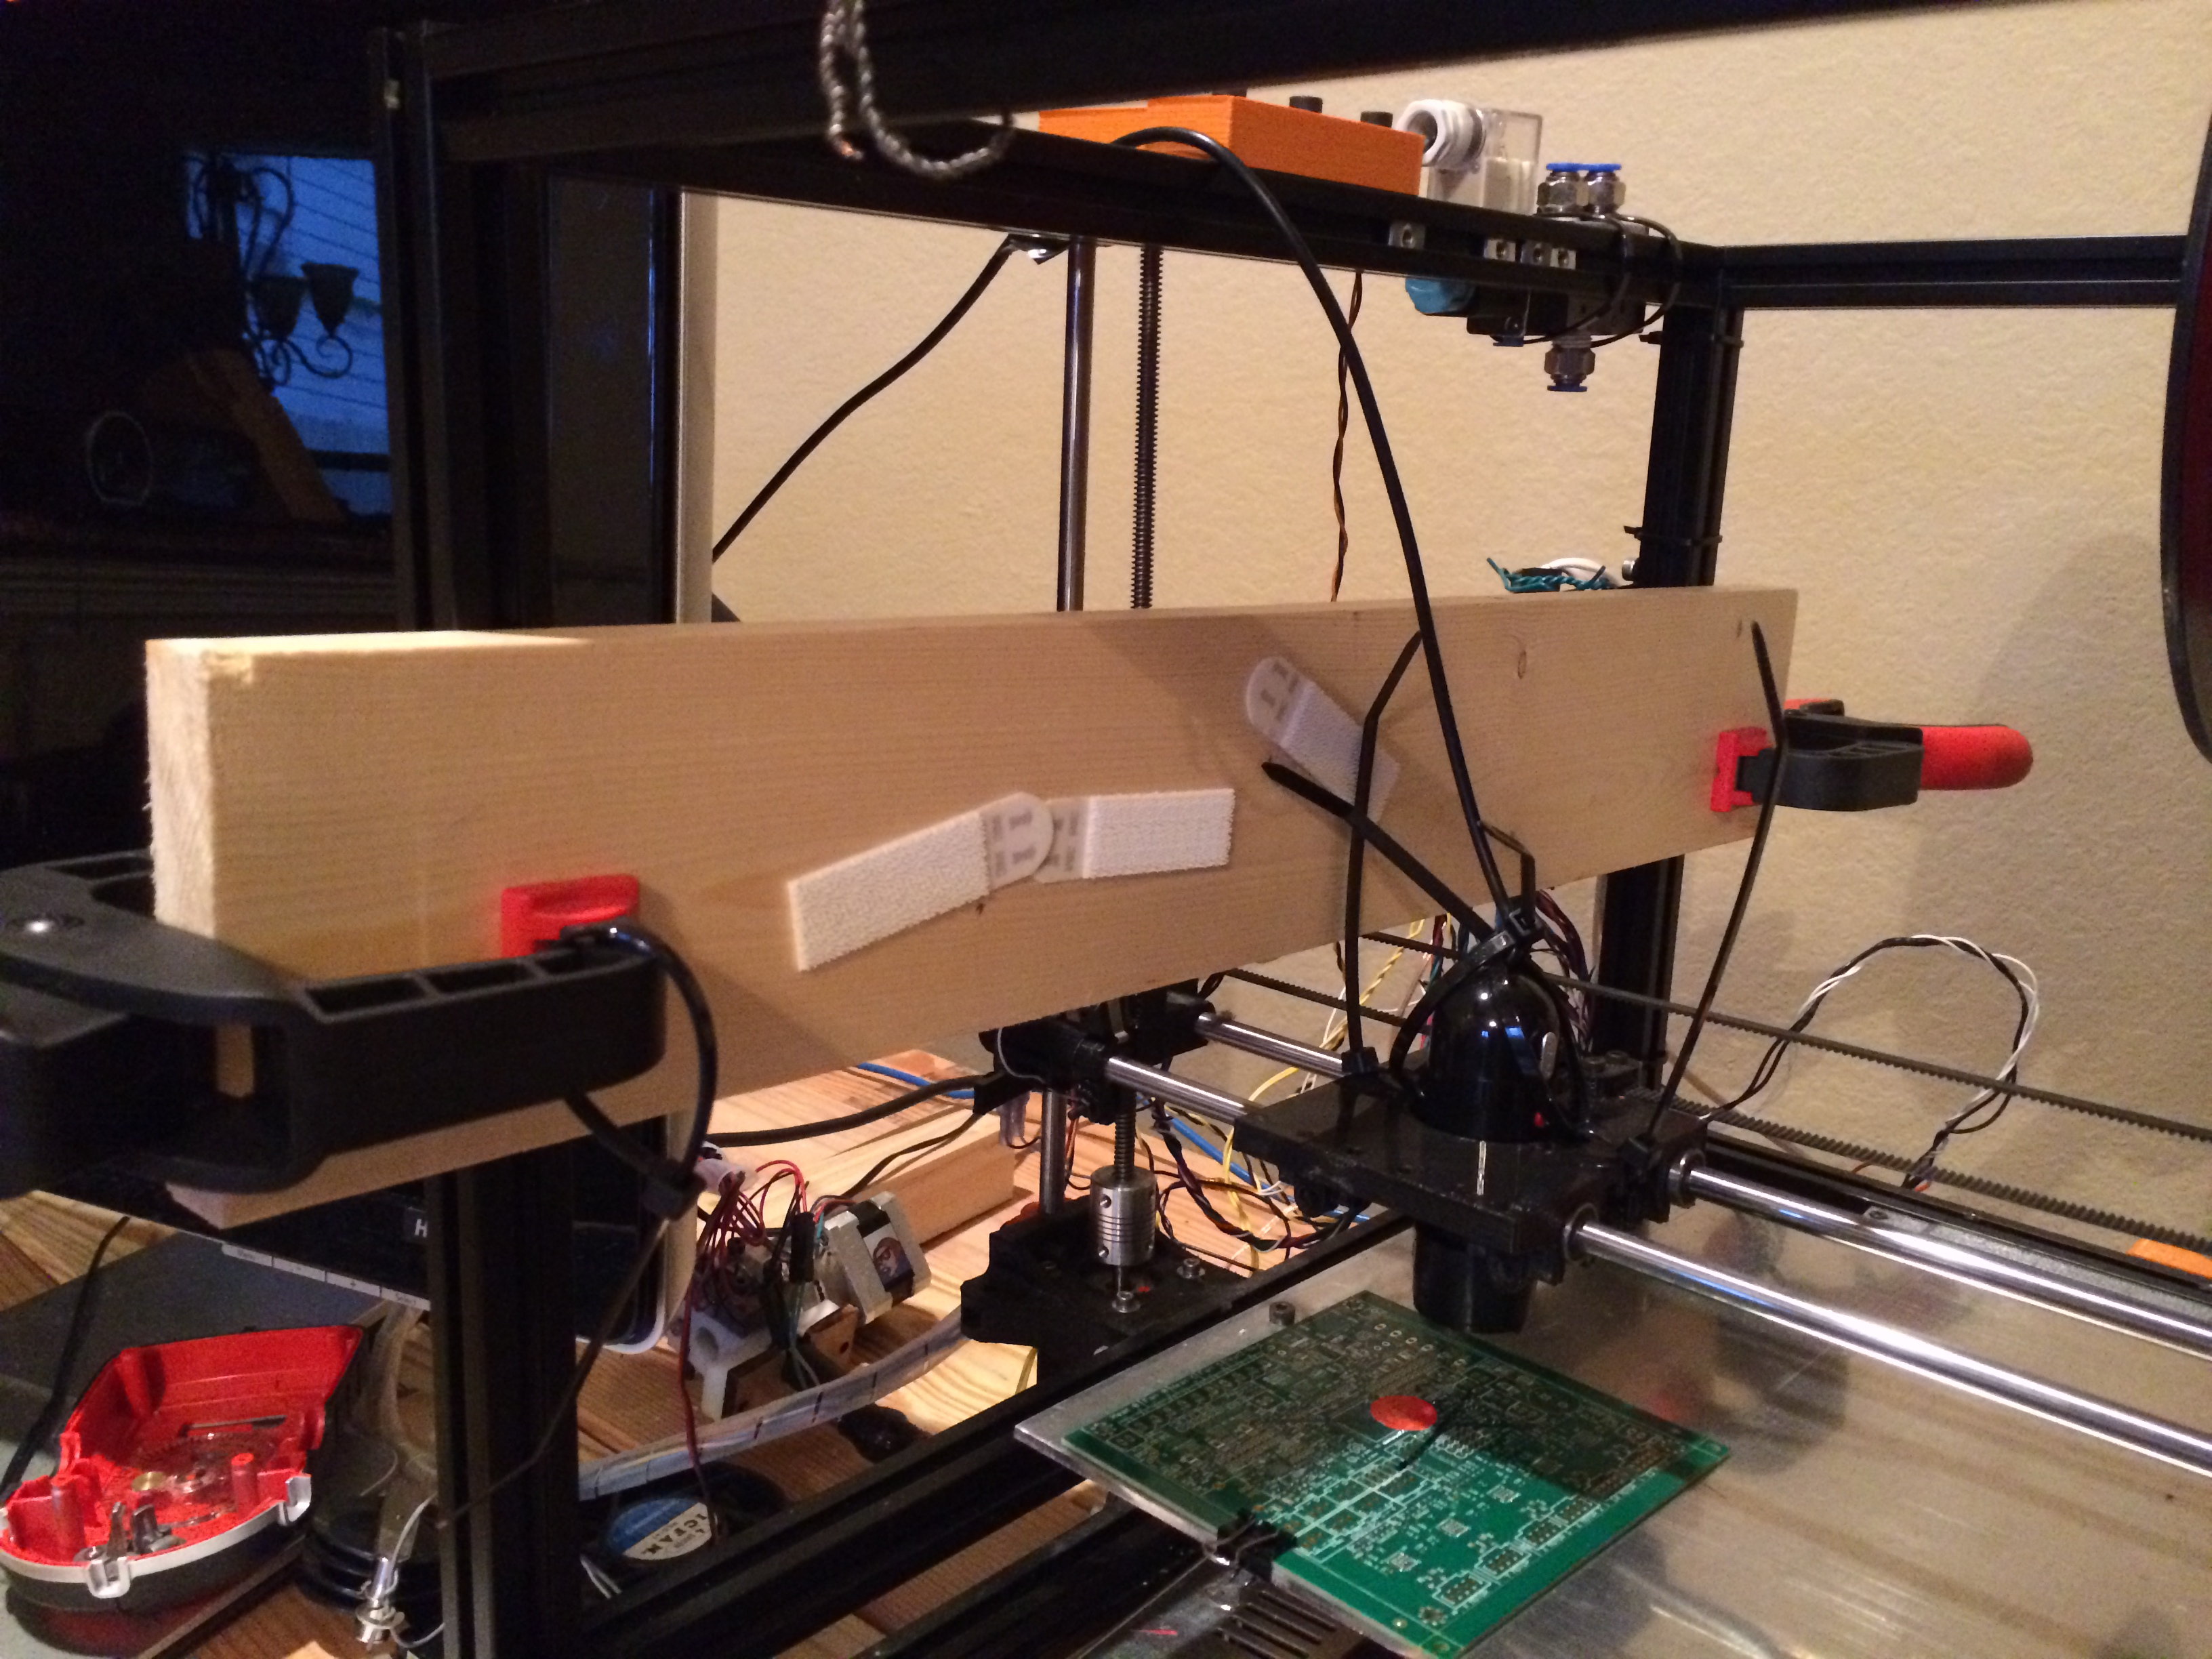
\includegraphics[scale=0.1,angle=270]{images/volume_analysis_setup/IMG_0614.JPG}
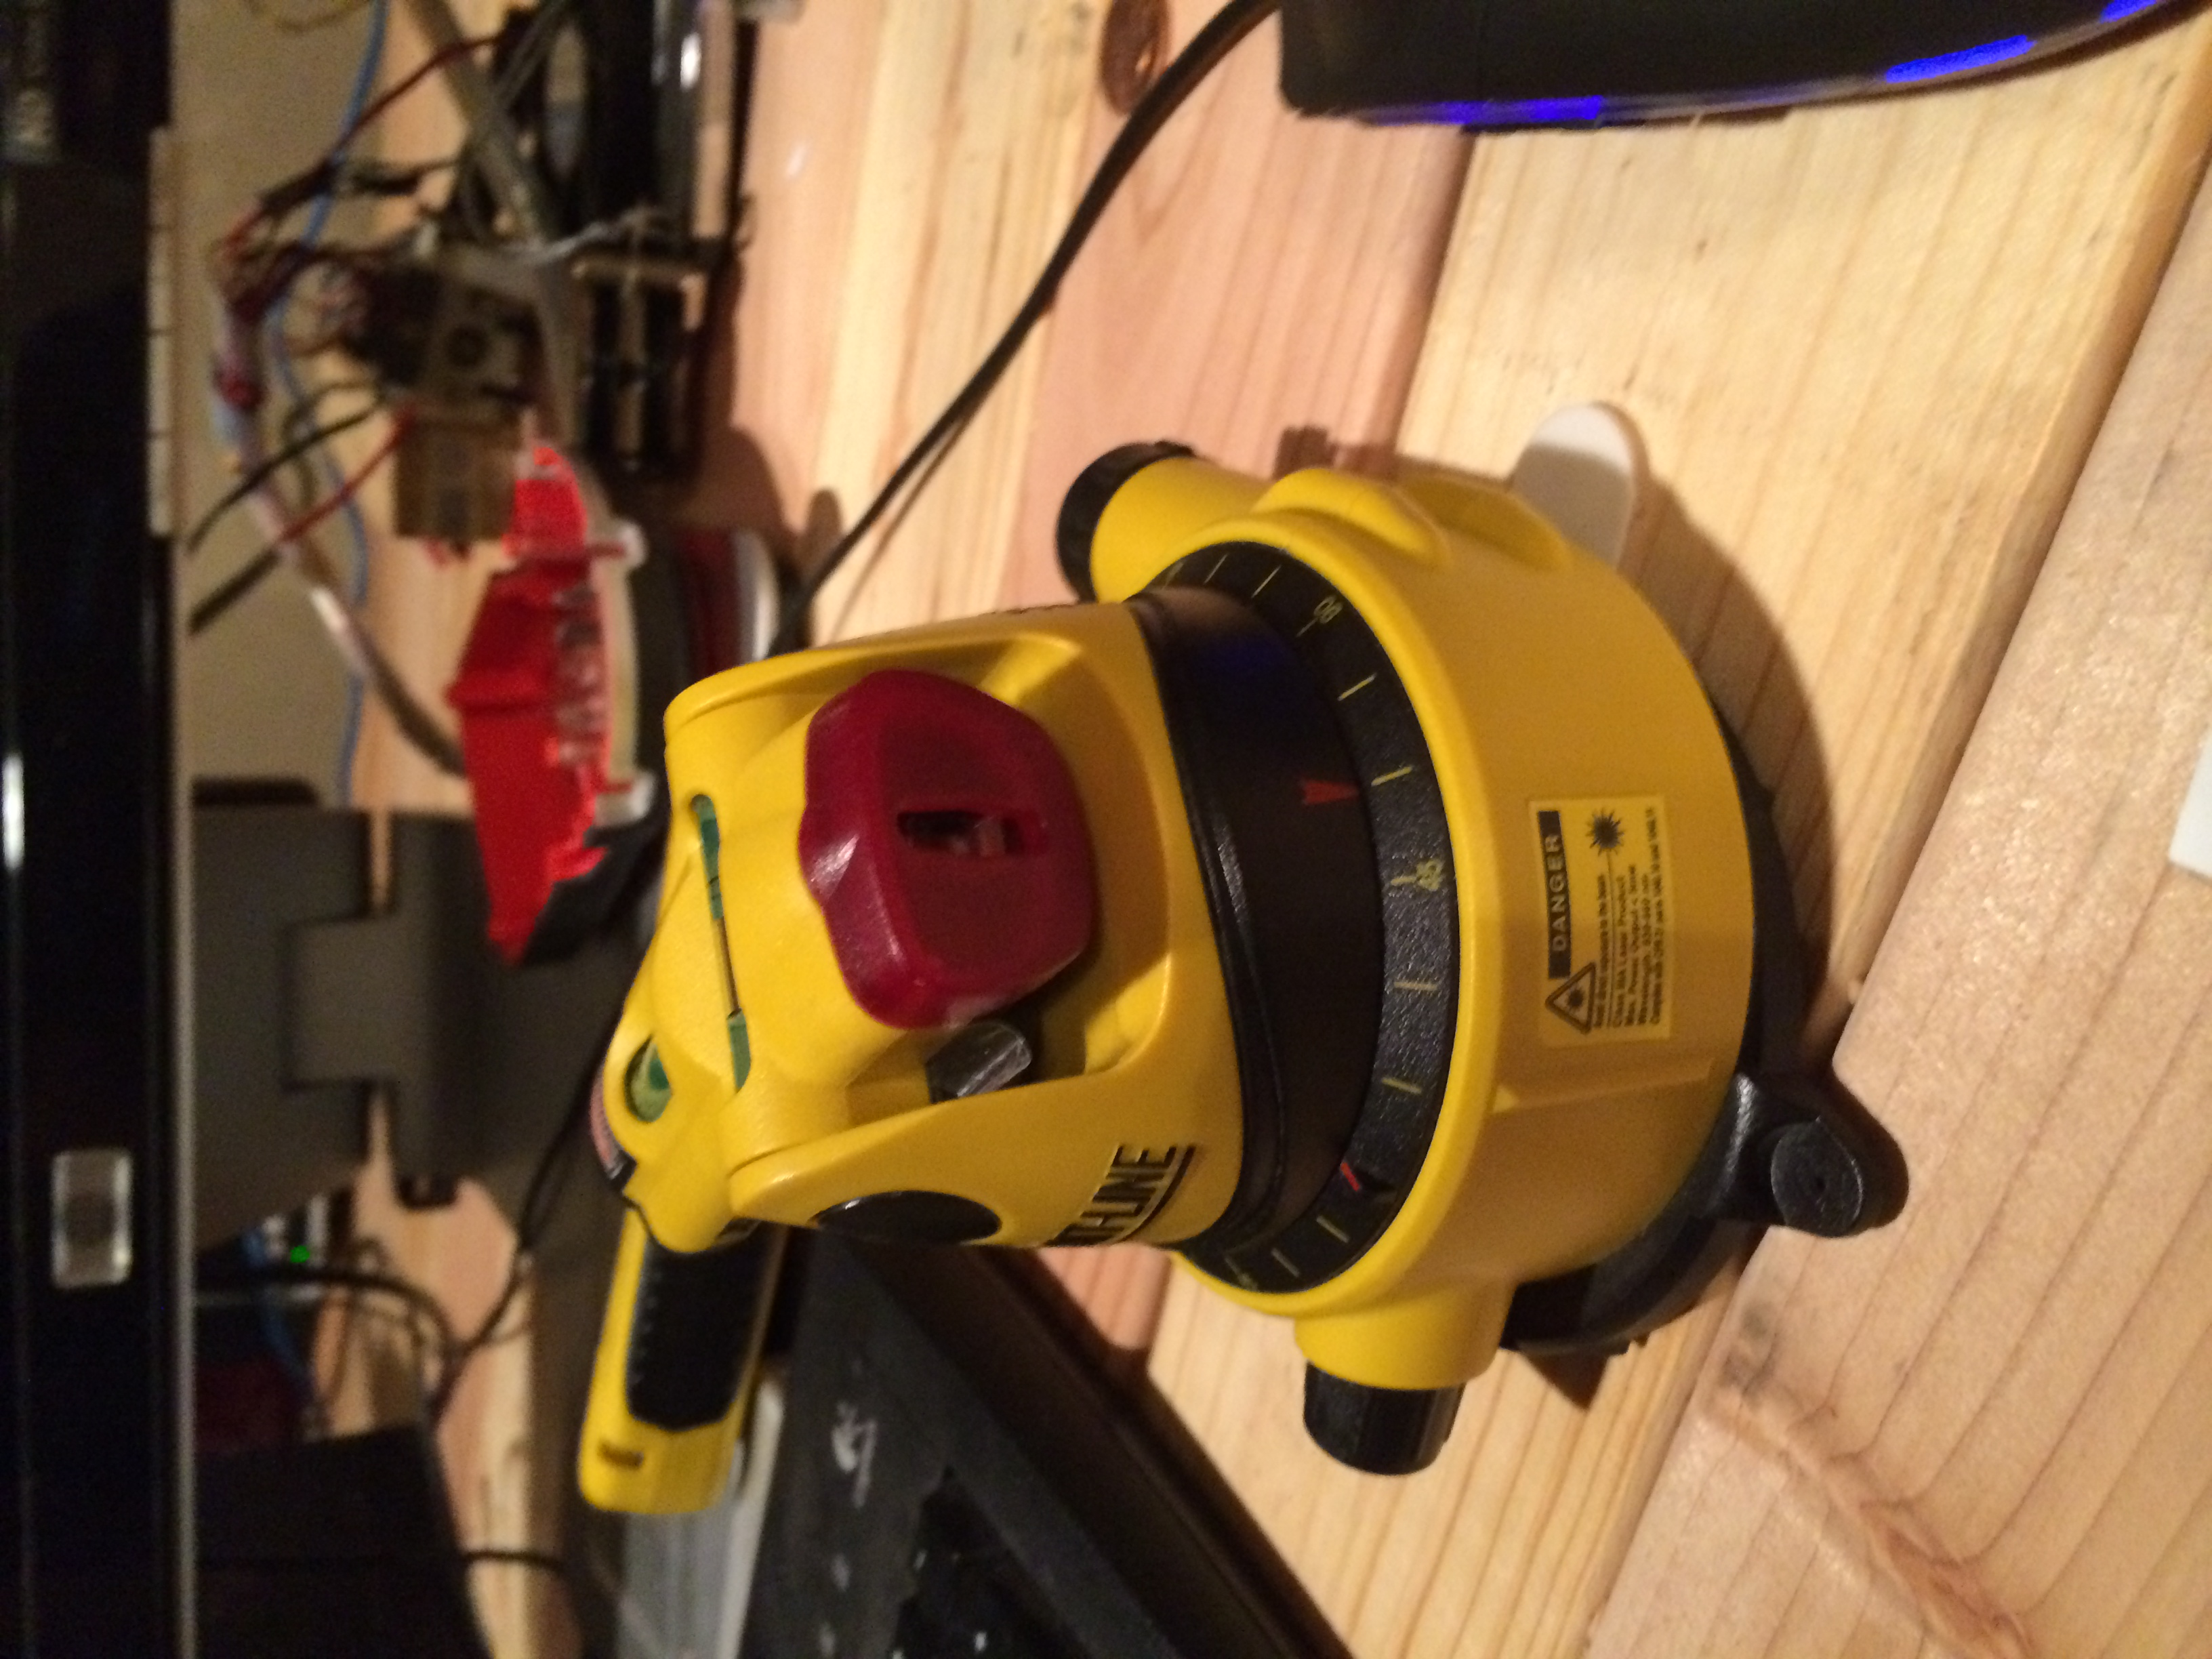
\includegraphics[scale=0.1,angle=270]{images/volume_analysis_setup/IMG_0616.JPG}
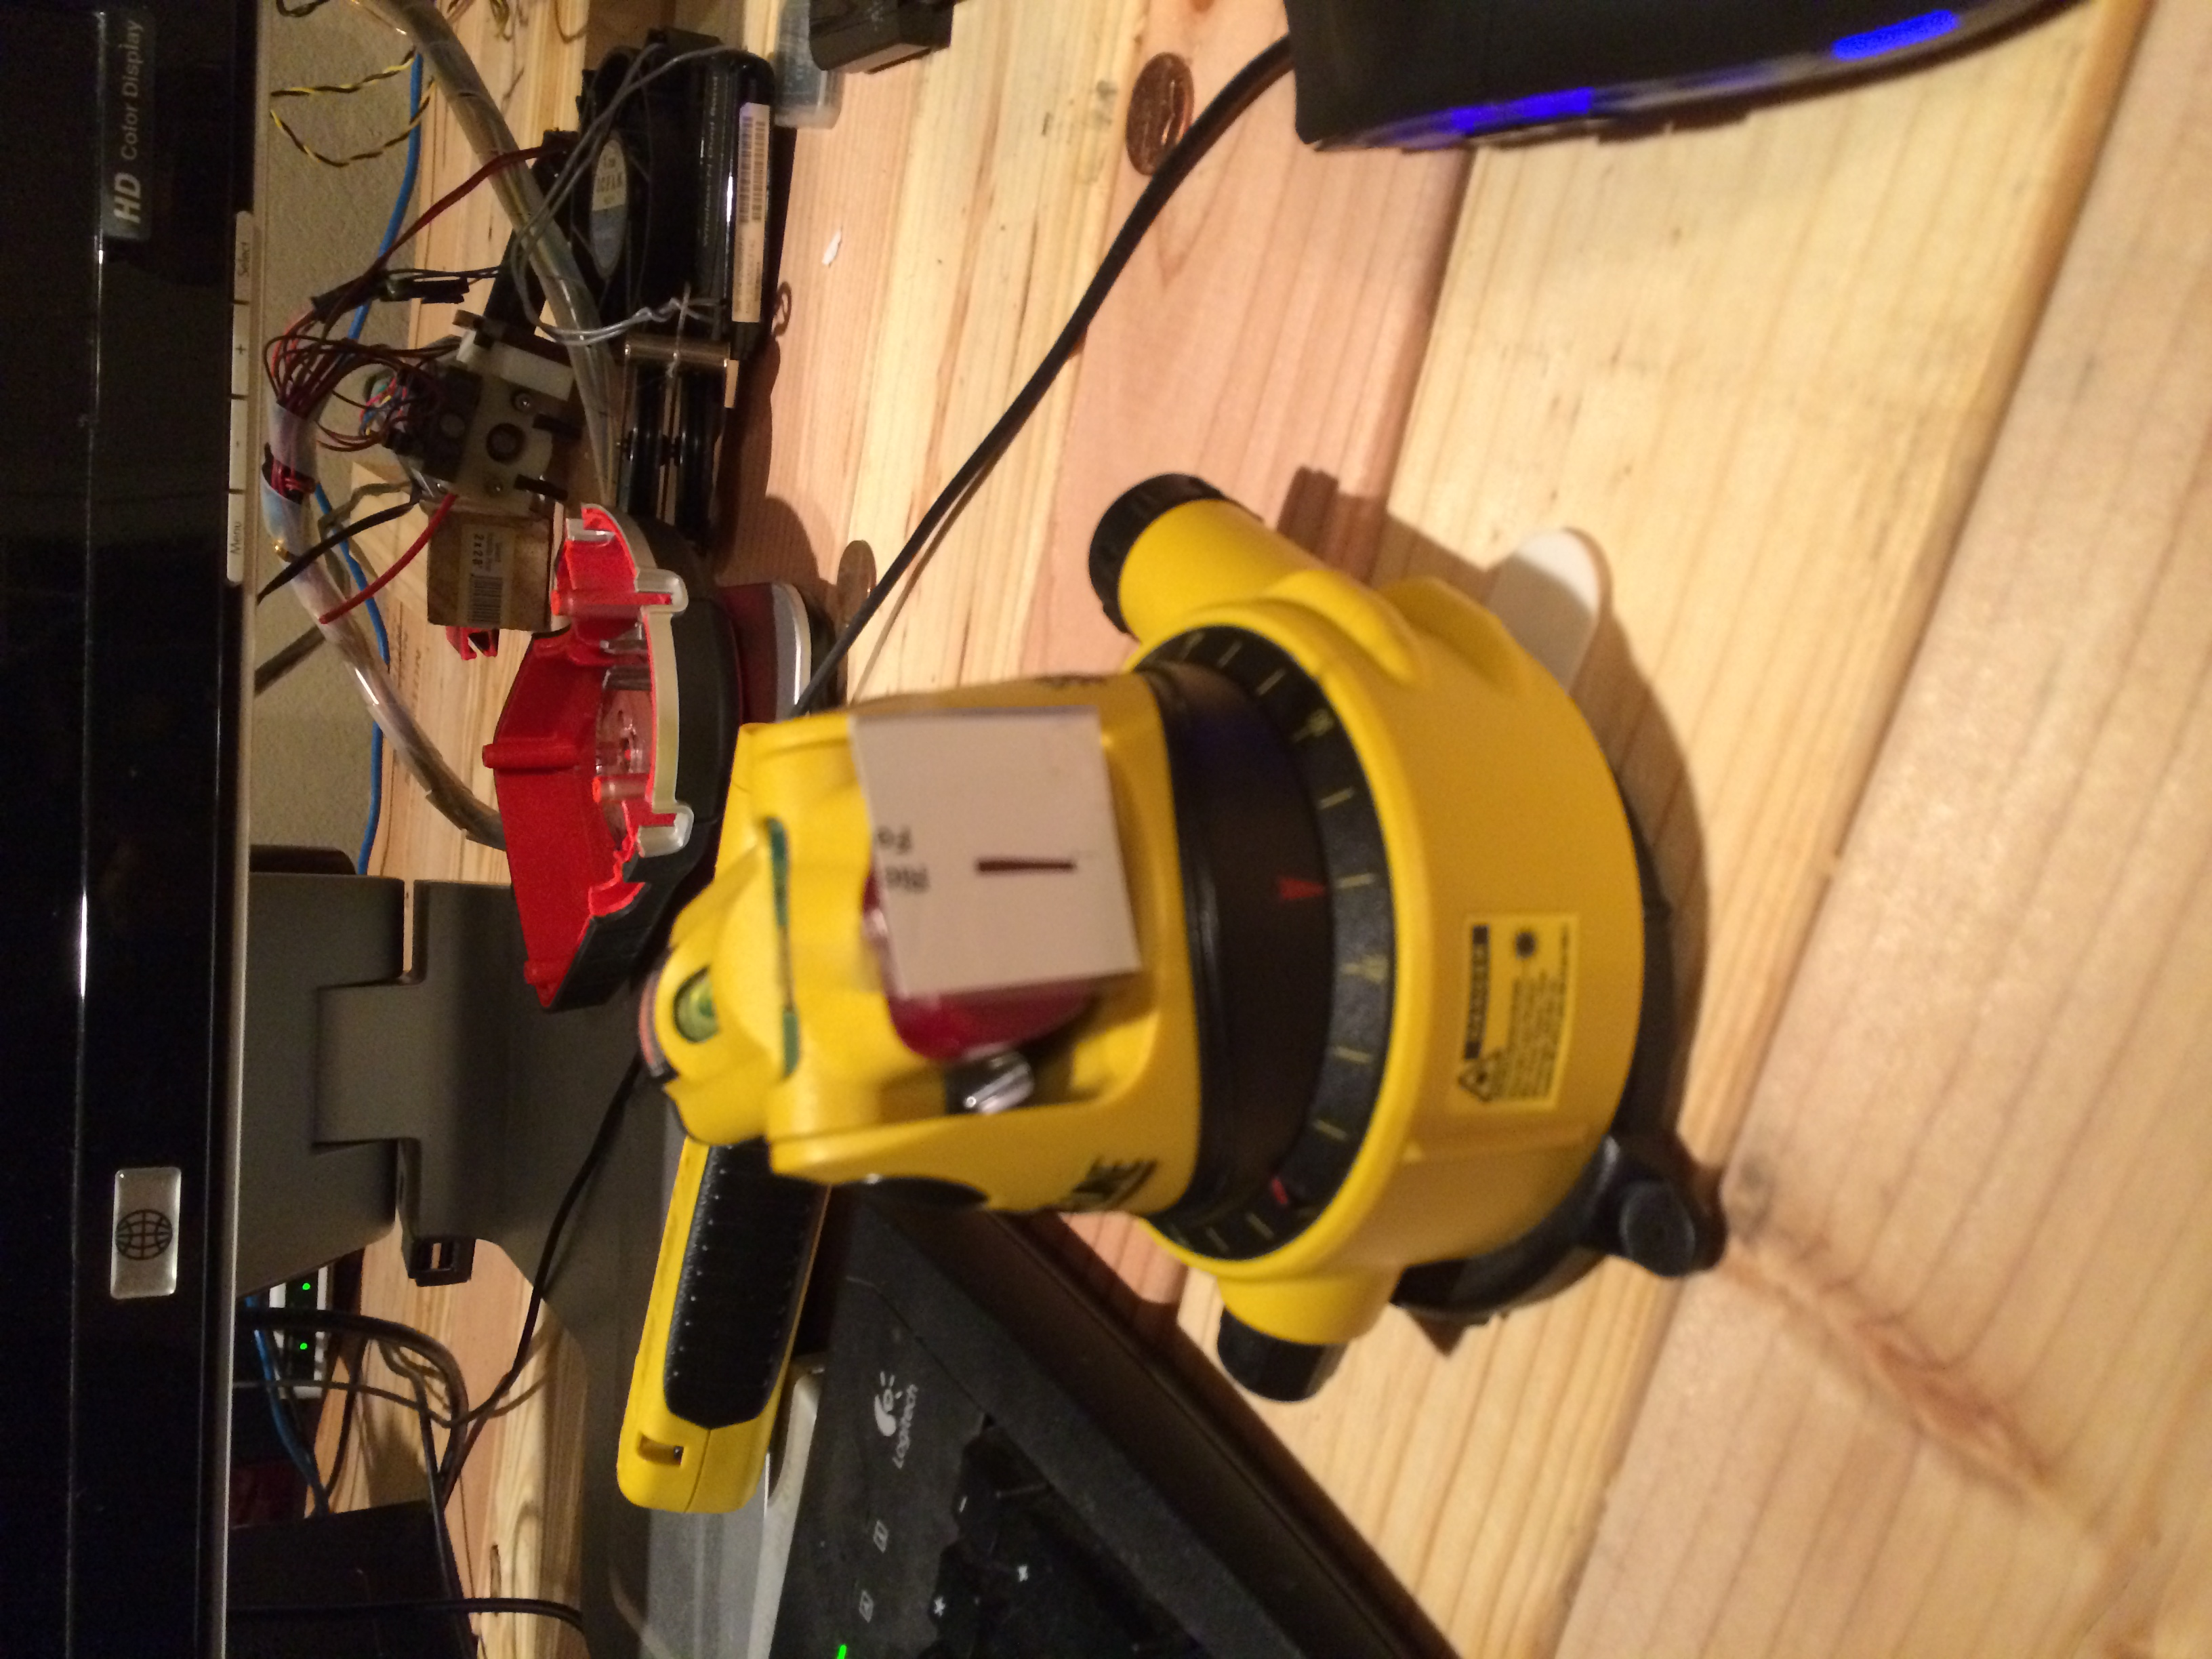
\includegraphics[scale=0.1,angle=270]{images/volume_analysis_setup/IMG_0617.JPG}
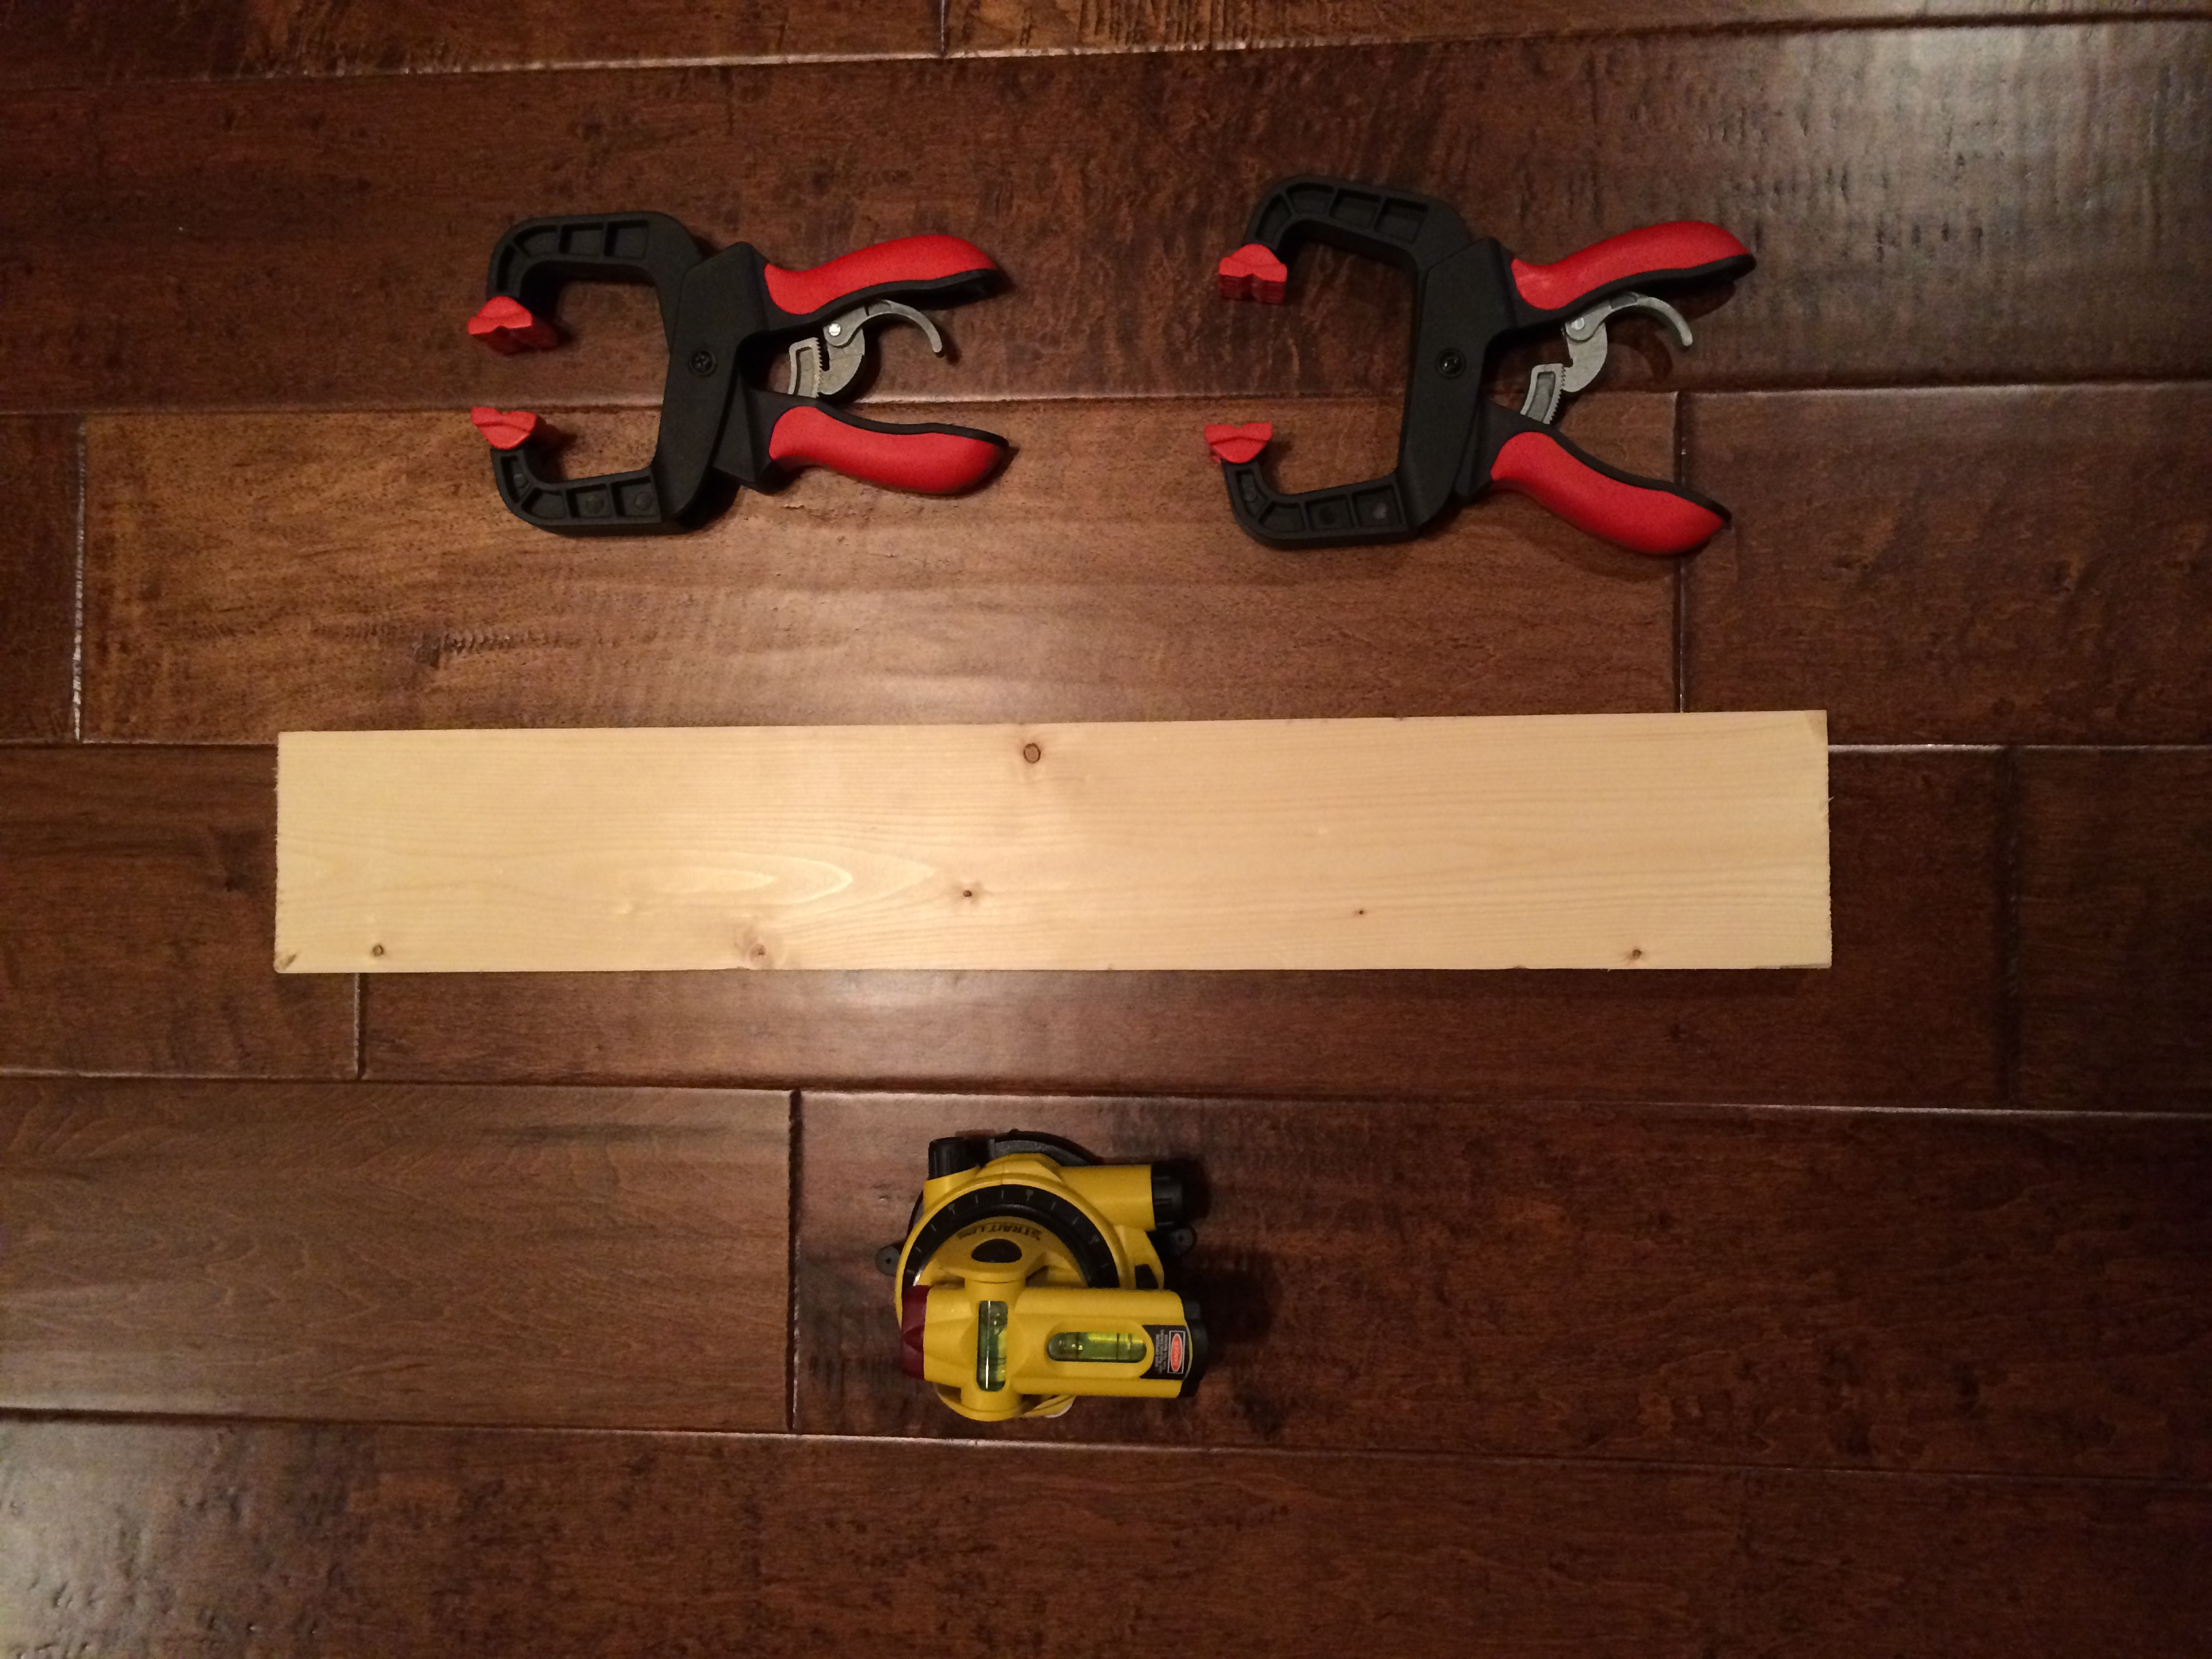
\includegraphics[scale=0.1,angle=270]{images/volume_analysis_setup/IMG_0618.JPG}
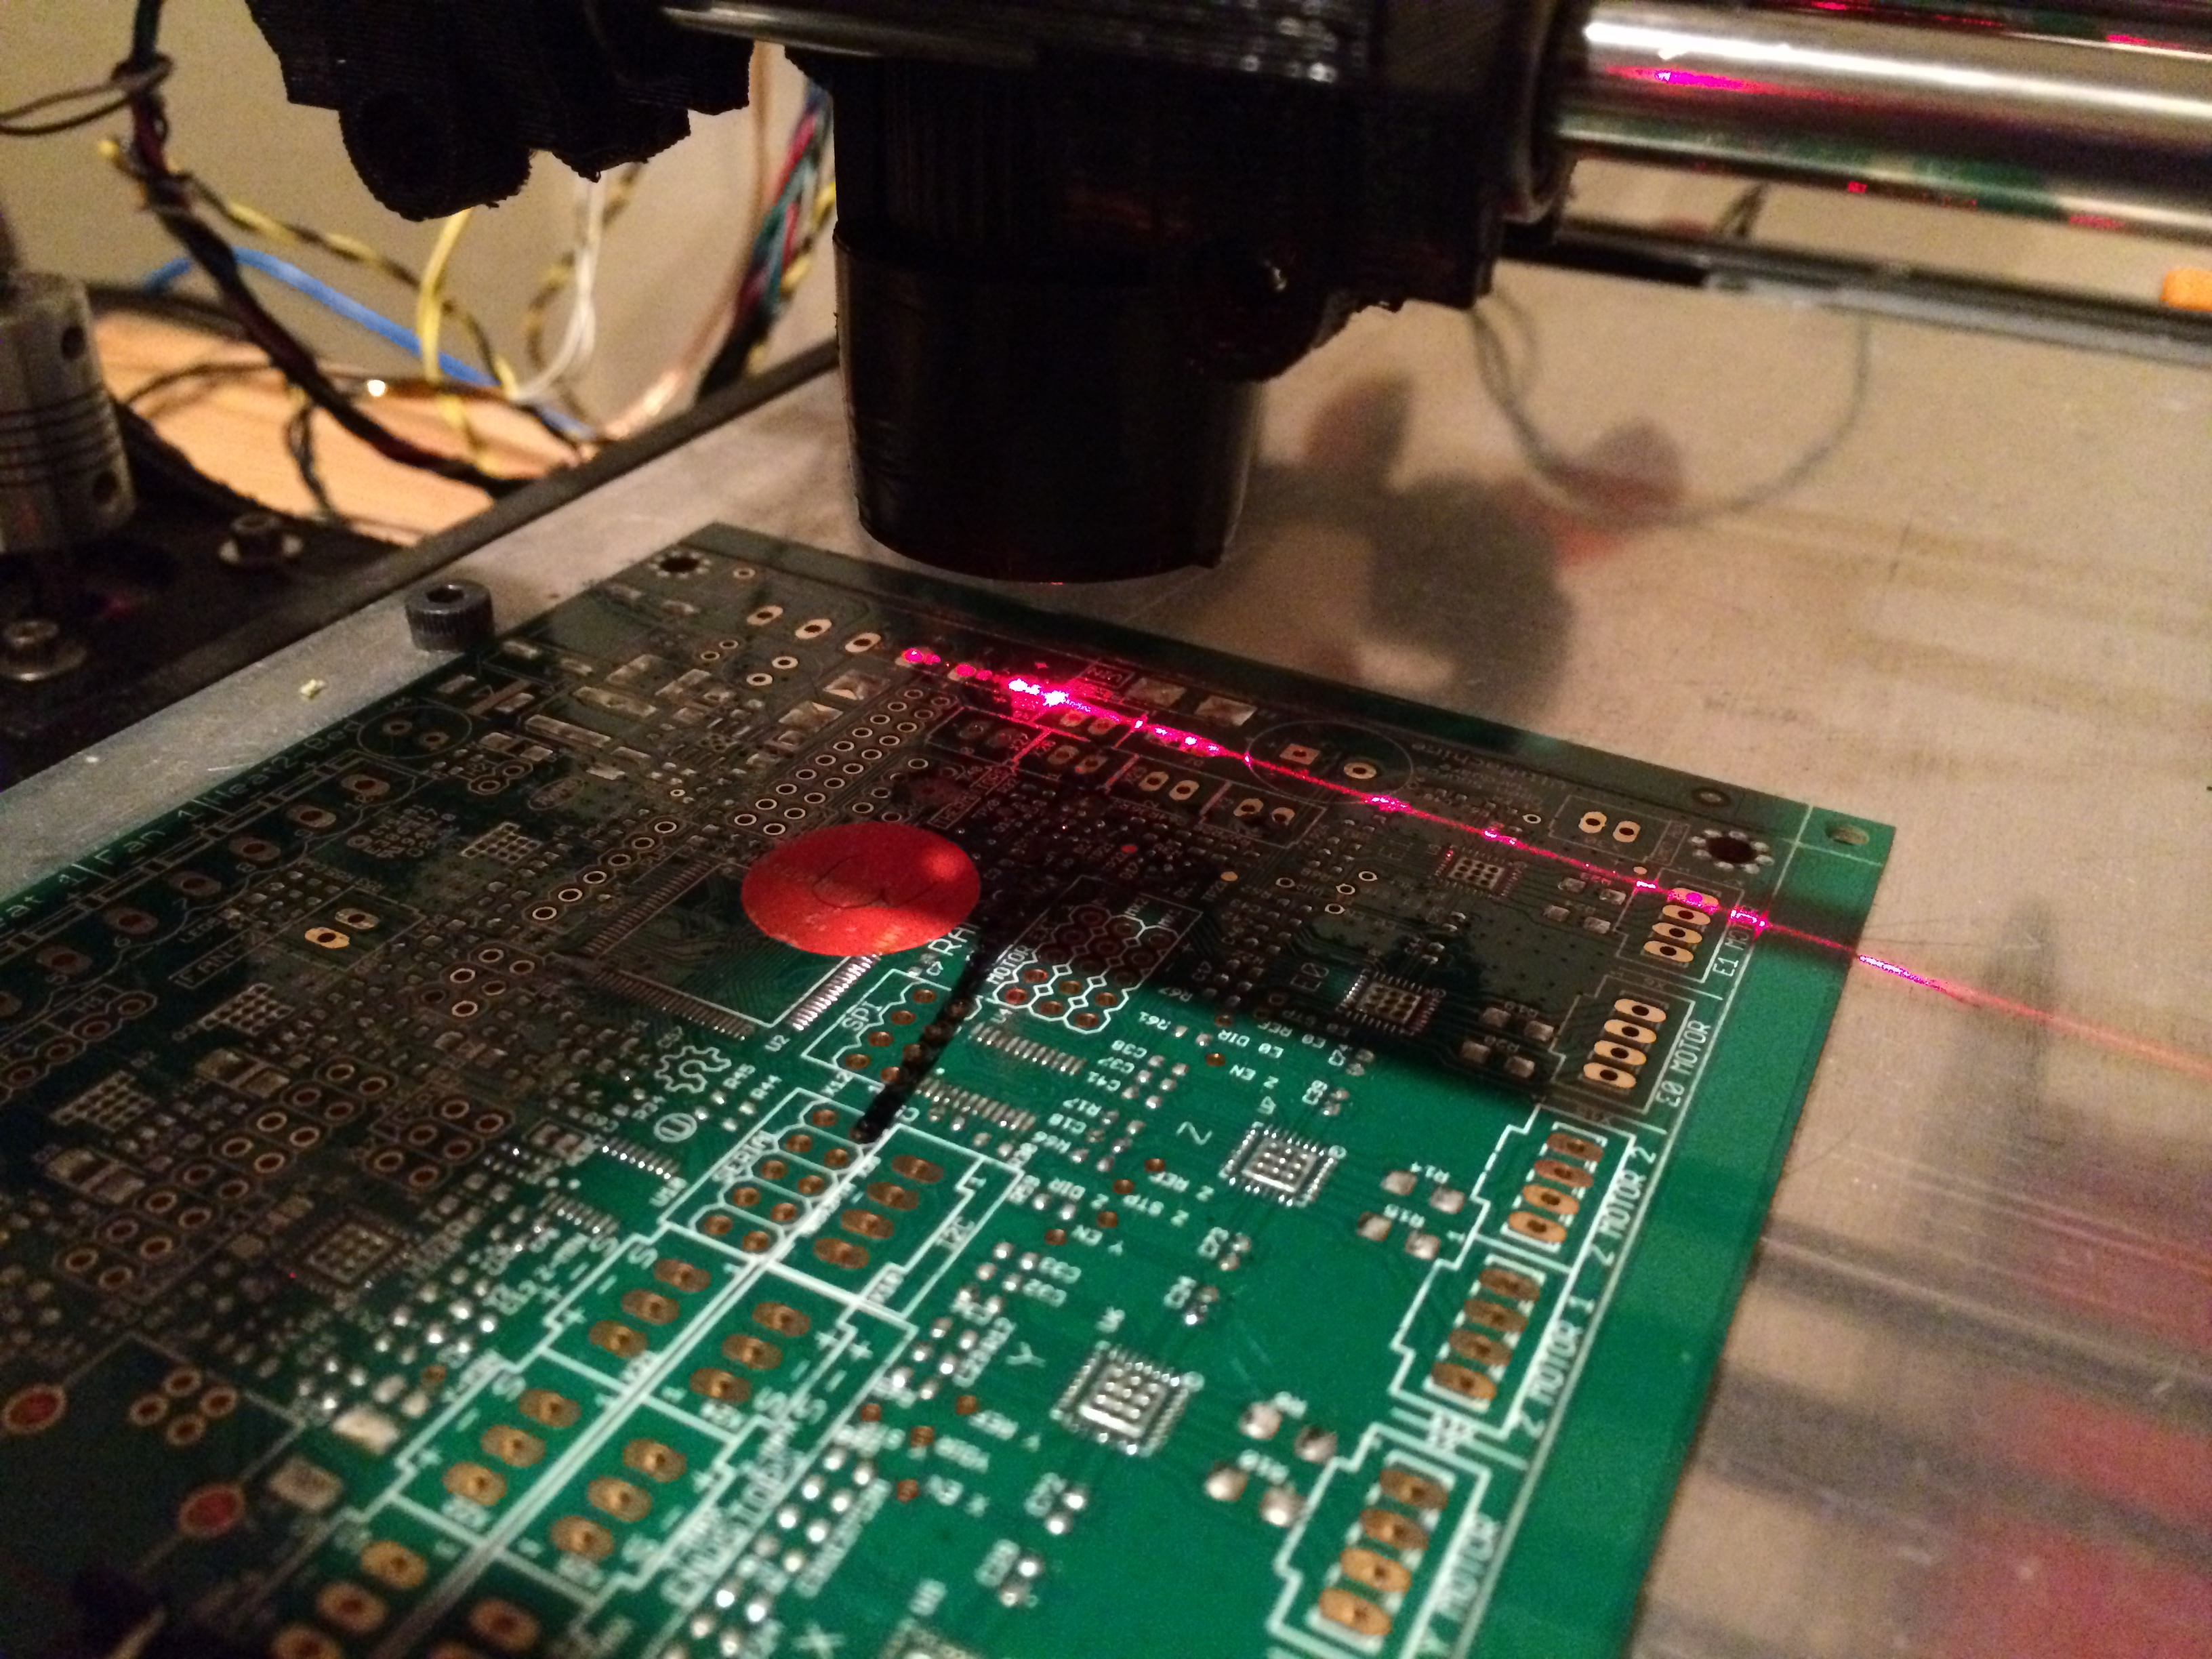
\includegraphics[scale=0.1]{images/volume_analysis_setup/IMG_0606.JPG}

\includegraphics{images/volume_analysis_setup/laser-8}


\section{Volume Image Processing}
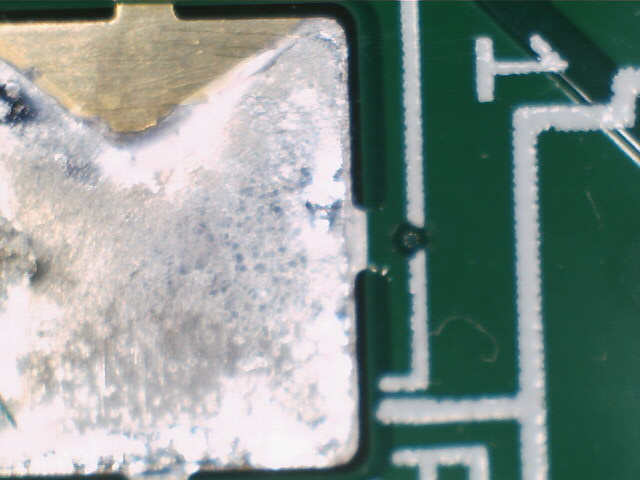
\includegraphics{images/volume_image_processing/led_image.png}
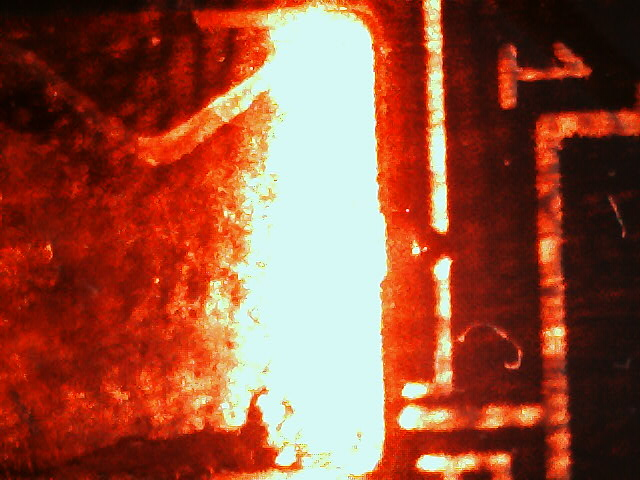
\includegraphics{images/volume_image_processing/laser_image.png}

\includegraphics{images/volume_image_processing/binary_led_image.png}

\includegraphics{images/volume_image_processing/binary_laser_image.png}

\includegraphics{images/volume_image_processing/union_laser_led_binaries.png}


\section{Volume Results}
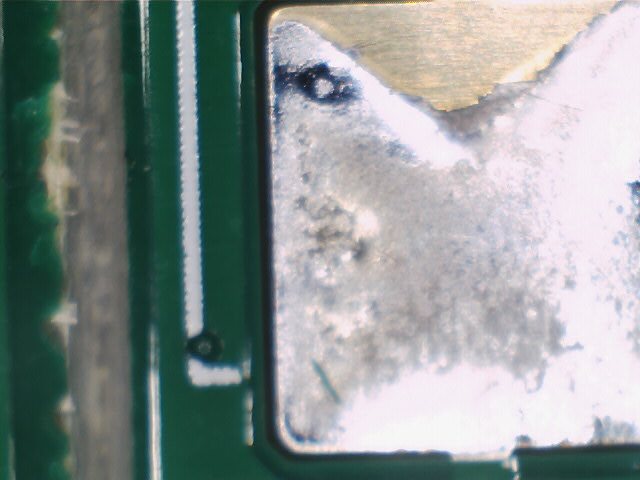
\includegraphics{images/volume_results/solder_led_hole.png}
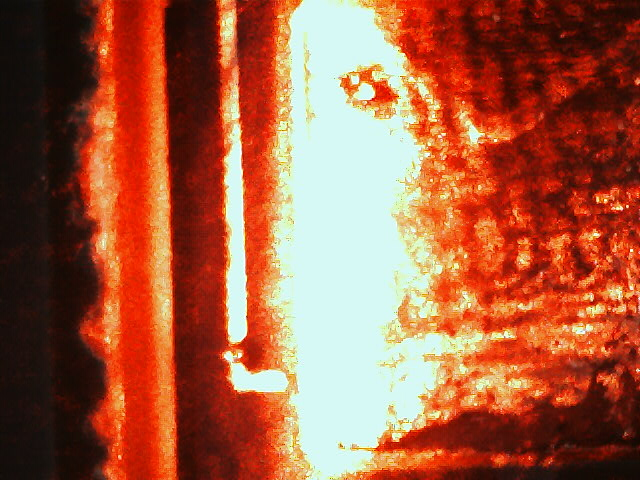
\includegraphics{images/volume_results/solder_laser_hole.png}
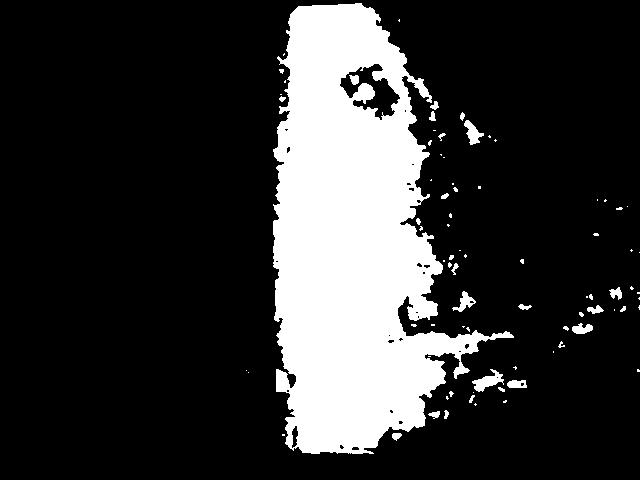
\includegraphics{images/volume_results/binary_image_hole.png}
Notice how the top of the white blob is thinner than the middle.  That is because the volume of solder at the top is less than the volume of solder at the middle. Also notice the black hole, this corresponds to a hole in the solder paste.

\section{Classification}
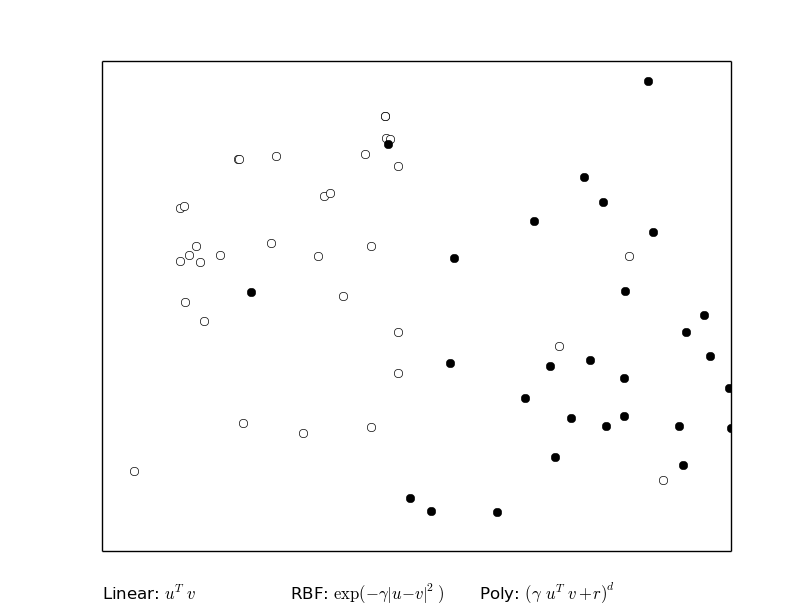
\includegraphics{images/Classification/data.png}
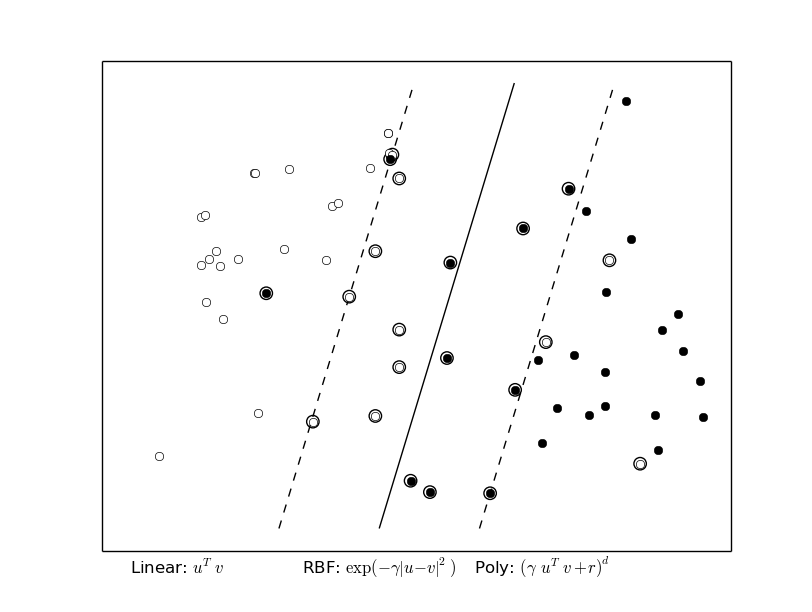
\includegraphics{images/Classification/analized_data.png}

%\begin{abstract}

%\end{abstract}


%\section{Introduction}
%Repeatability and accuracy is essential to PCB manufacturing.  That is why careful inspection %of PCB boards is an integral component of the PCB manufacturing process.  It is also essential %to 3D printing.  As 3D printing technology becomes more common place 

%\paragraph{Outline}
%The remainder of this article is organized as follows.
%Section~\ref{previous work} gives account of previous work.
%Our new and exciting results are described in Section~\ref{results}.
%Finally, Section~\ref{conclusions} gives the conclusions.

%\section{Previous work}\label{previous work}
%A much longer \LaTeXe{} example was written by Gil~\cite{Gil:02}.

%\section{Results}\label{results}
%In this section we describe the results.

%\section{Conclusions}\label{conclusions}
%We worked hard, and achieved very little.

%\bibliographystyle{abbrv}
%\bibliography{main}

\end{document}
